\input preamble.tex
\noindent
\begin{center}
{\bf Oversikt over stasjoner hos 3AUA Gand VGS }
\end{center}
\vskip 5pt
\section{Stasjon 01}

$$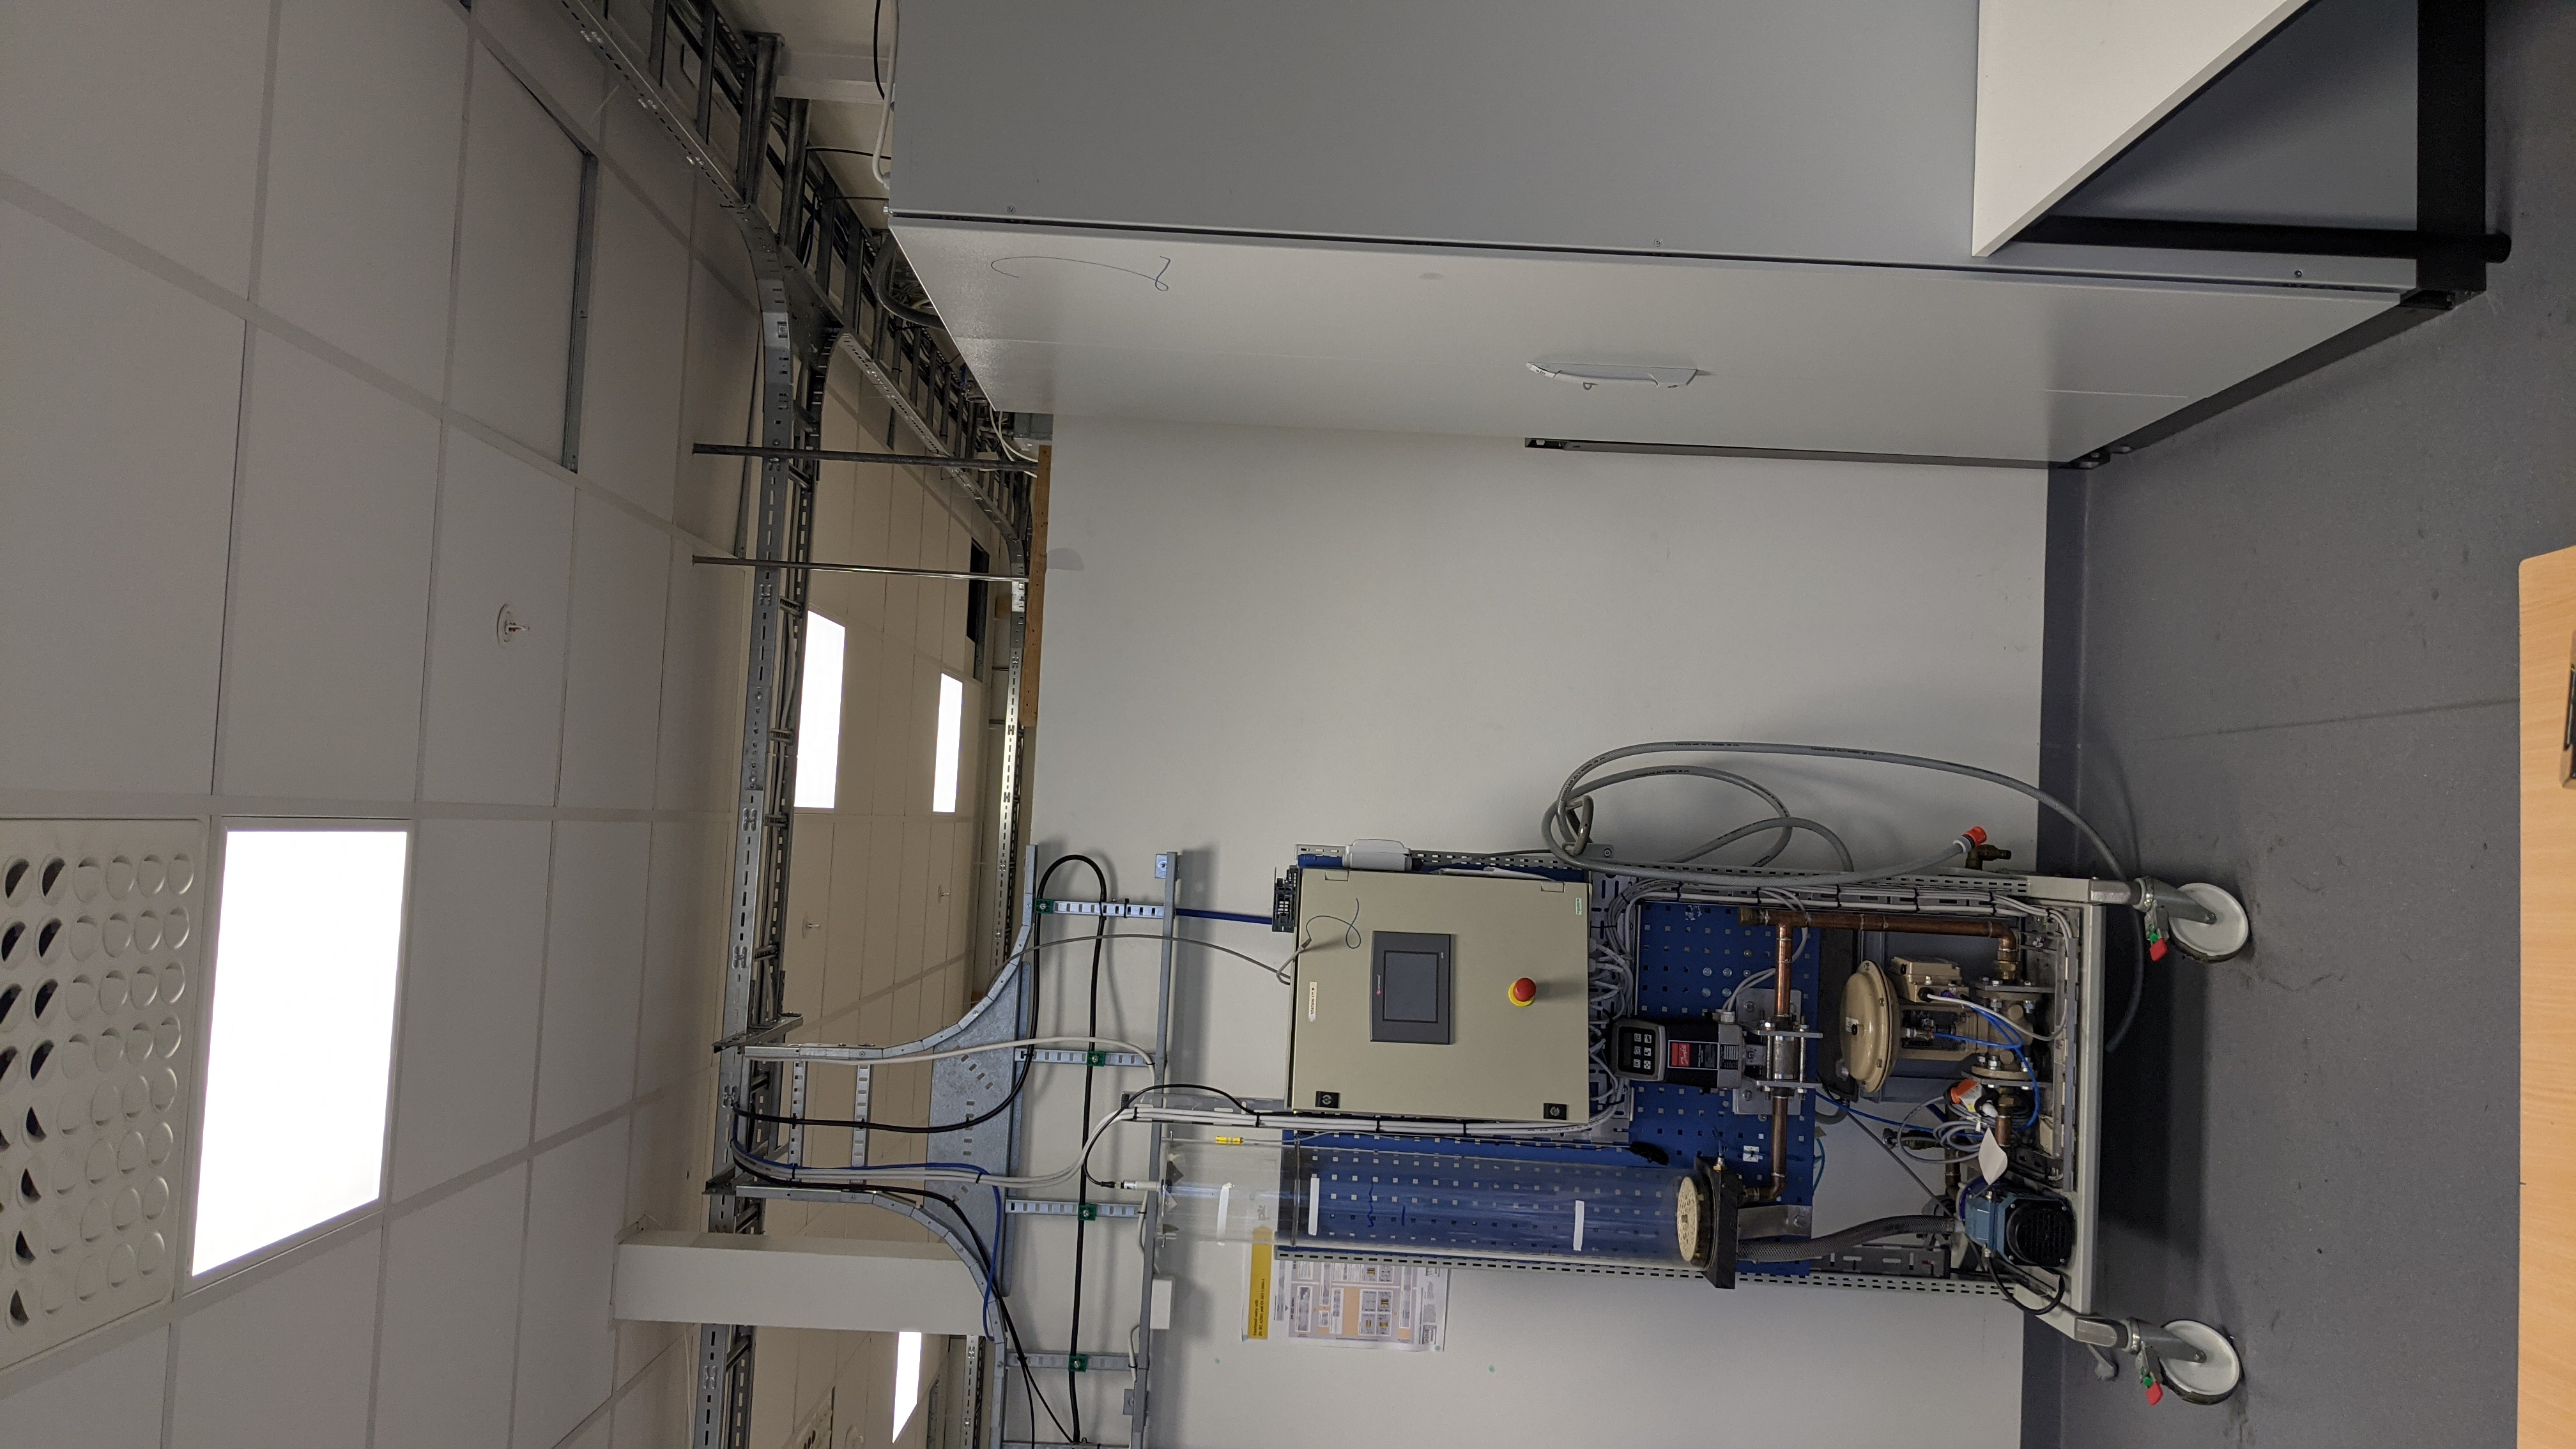
\includegraphics[width=10.5cm,angle=-90]{stasjon02x01.jpg}$$

Stasjon01 - Gandsfjorden Gondol er den første stajsonen vi starter med etter vi er fredige med repitisjon. Det er også den eneste stasjonen der hele klassen jobber med det samme. \\

Hensikten med denne stasjonen er å repitere grunnleggende koblingskunnskap i automasjonsfaget, gjøre elevene kjent med hvordan vi dokumenterer anlegg i 3AUA og bli kjent med PLS programmeringsverktøyet Codesys som vi bruker. 
\section{Stasjon 02}

$$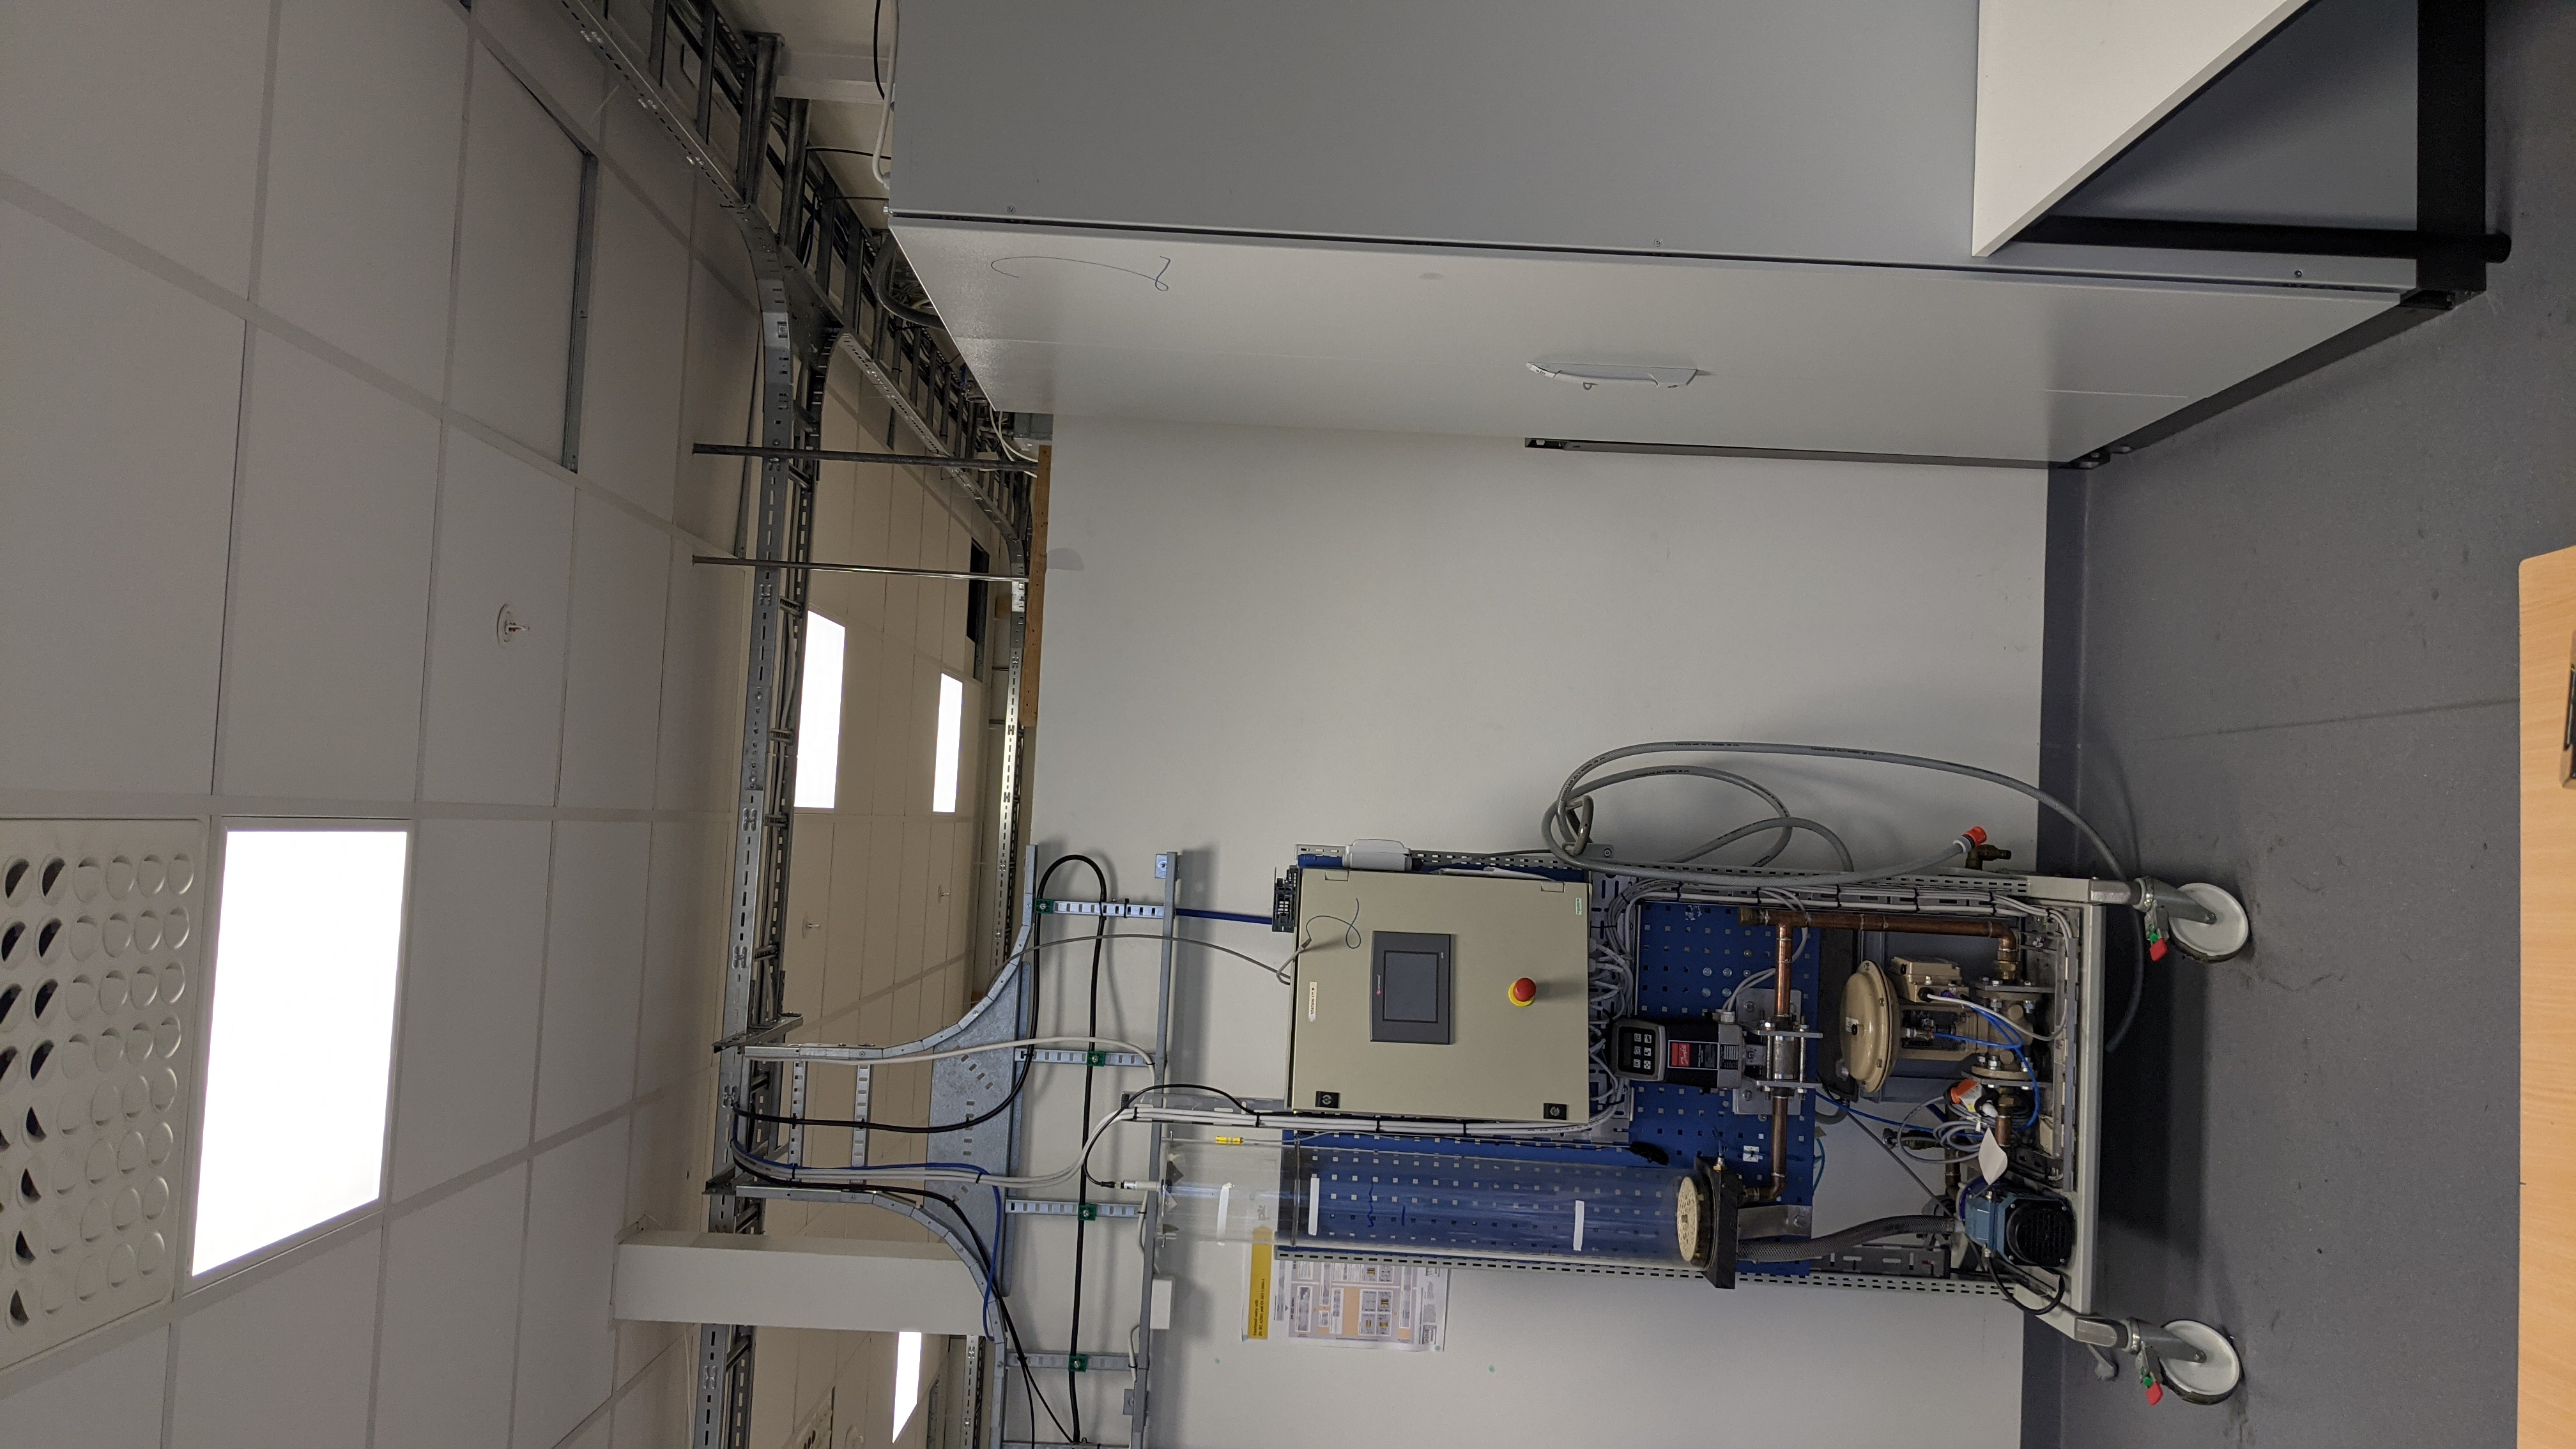
\includegraphics[width=10.5cm,angle=-90]{stasjon02x01.jpg}$$
Stasjon 02 består av et stort styreskap laget for å styre 5 ulike maskiner, med og uten EXi signaler. Detter er en stasjoner som er under oppbygning. Det er meningen å koble flere og flere stasjoner til  styreskapet. \\




\section{Stasjon 03}

$$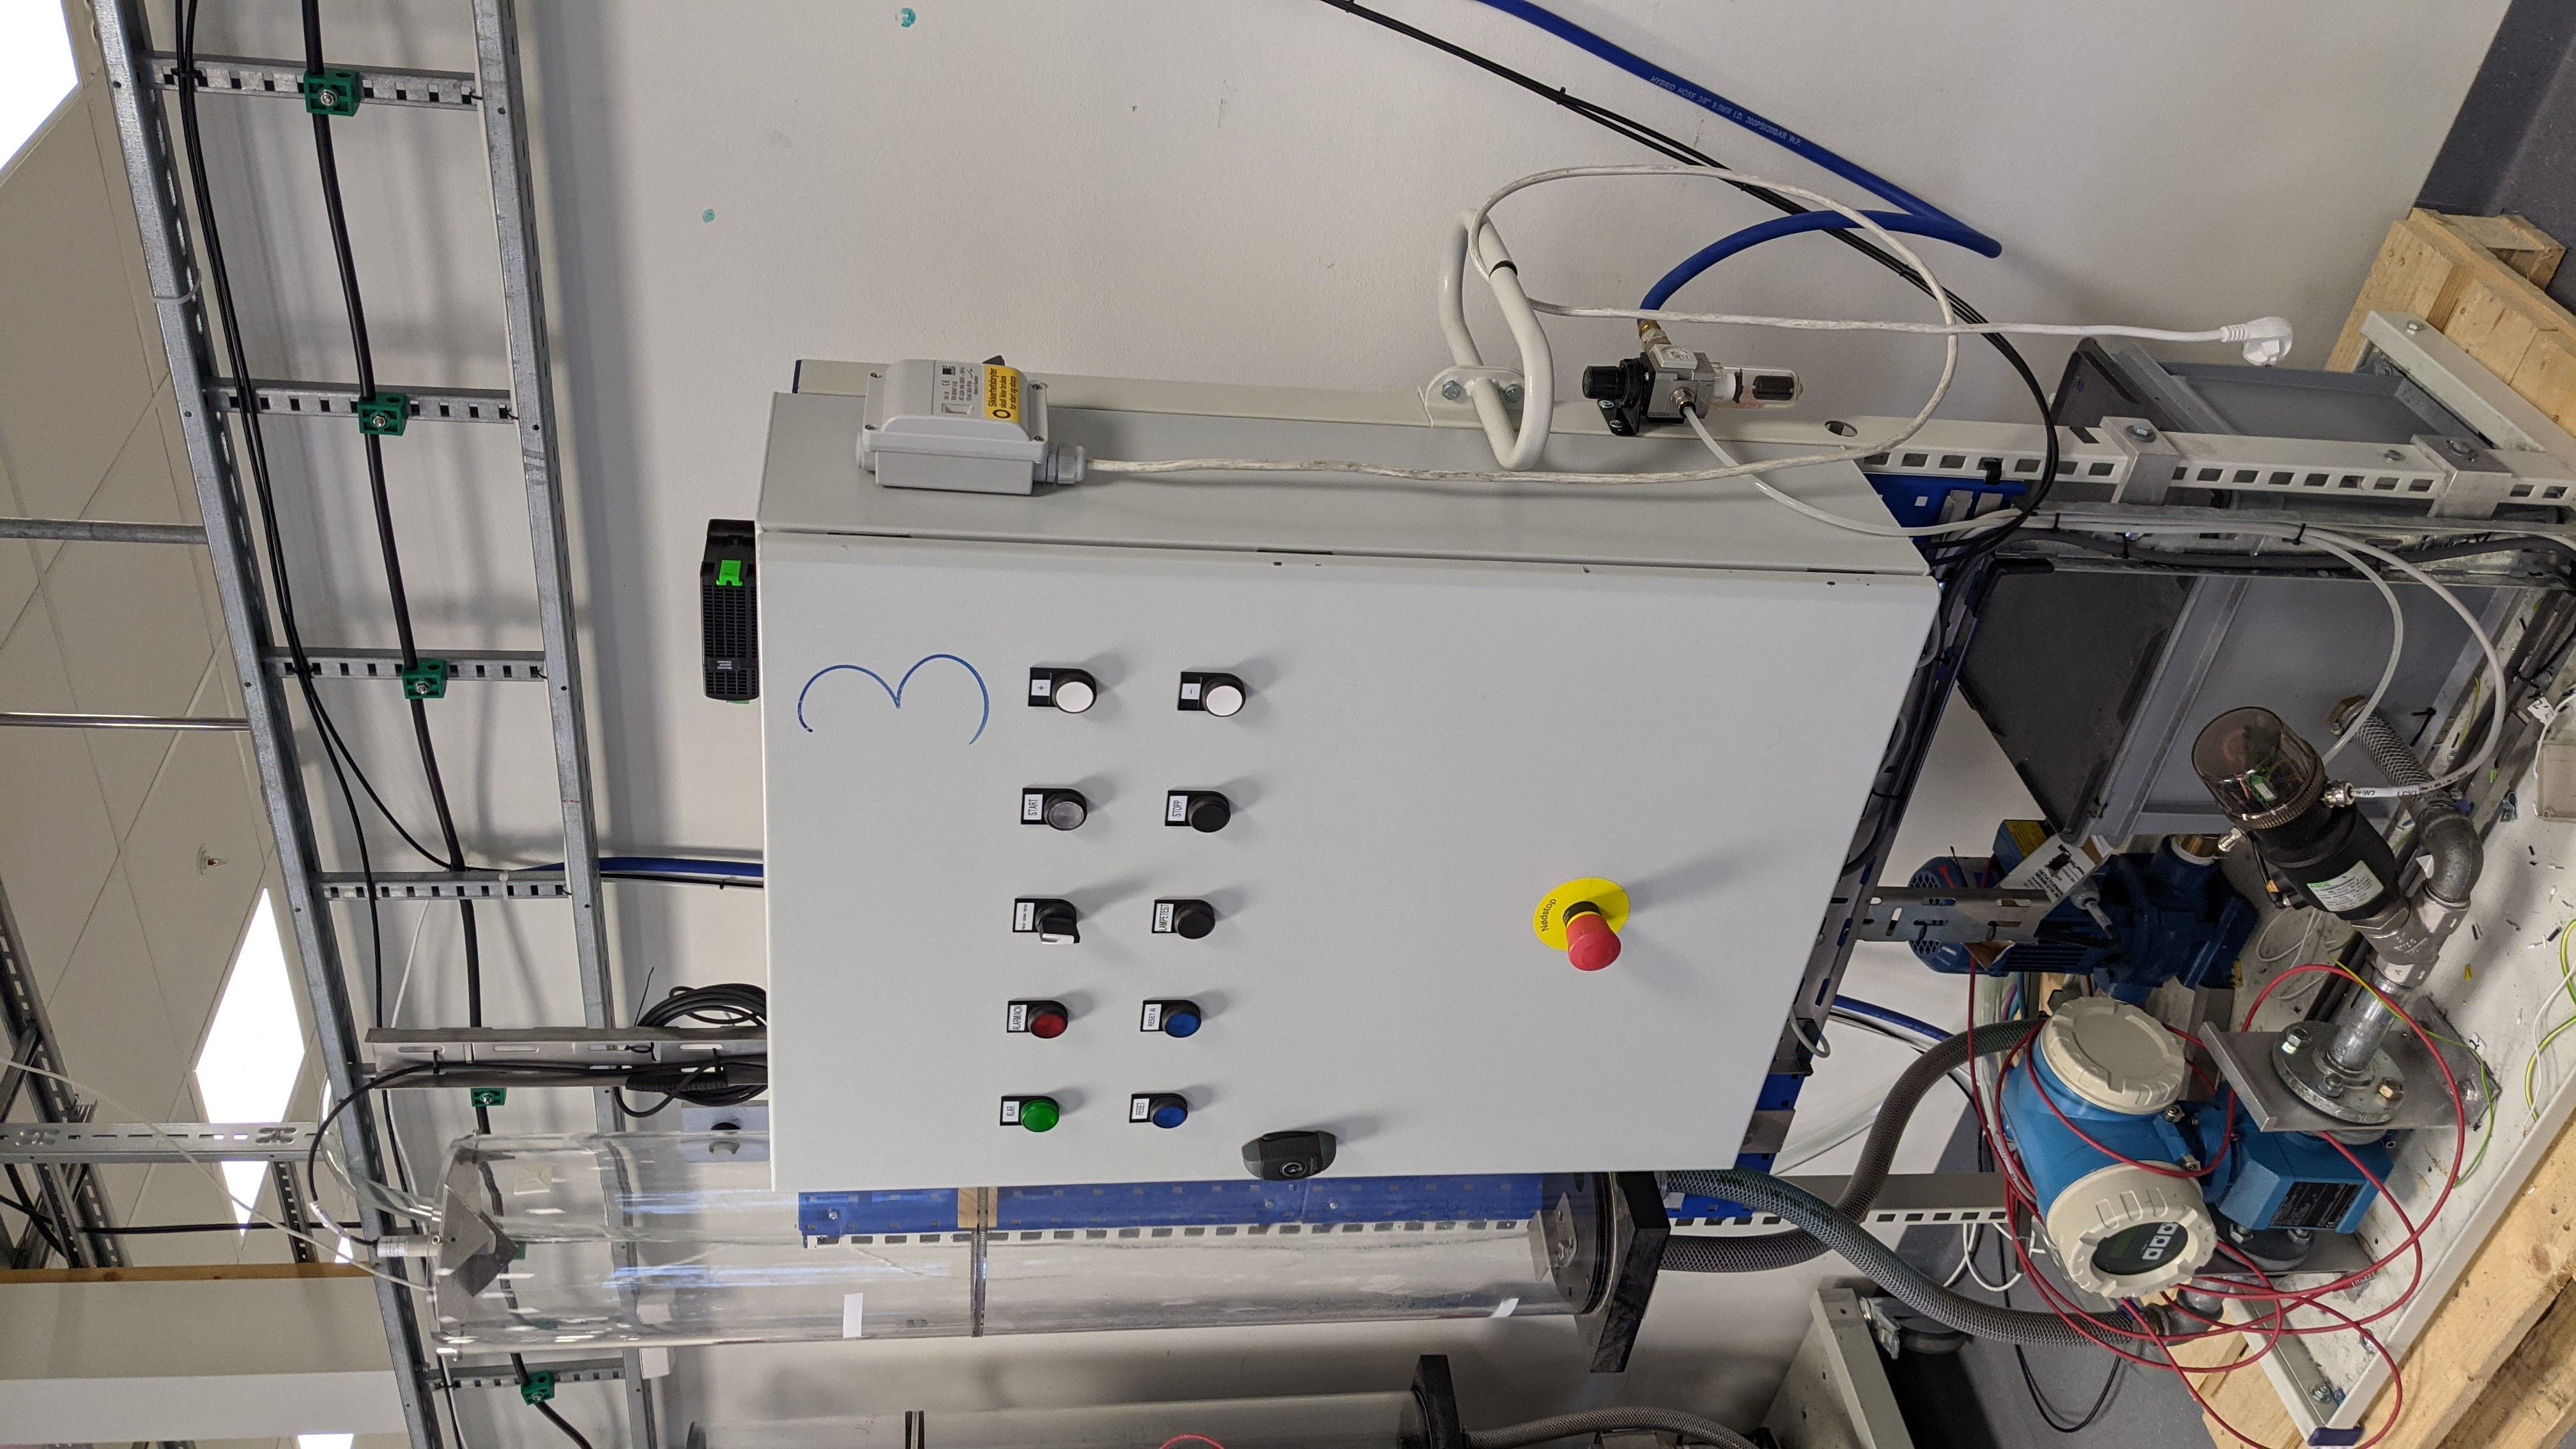
\includegraphics[width=10.5cm,angle=-90]{stasjon03x01.jpg}$$

Stasjon 03 er en Gand regueringsstasjon. Den er bygget for å kunne øve på ulike typer regulering. Dennestasjonen brukes for koblingsøvelser.

\section{Stasjon 04}

$$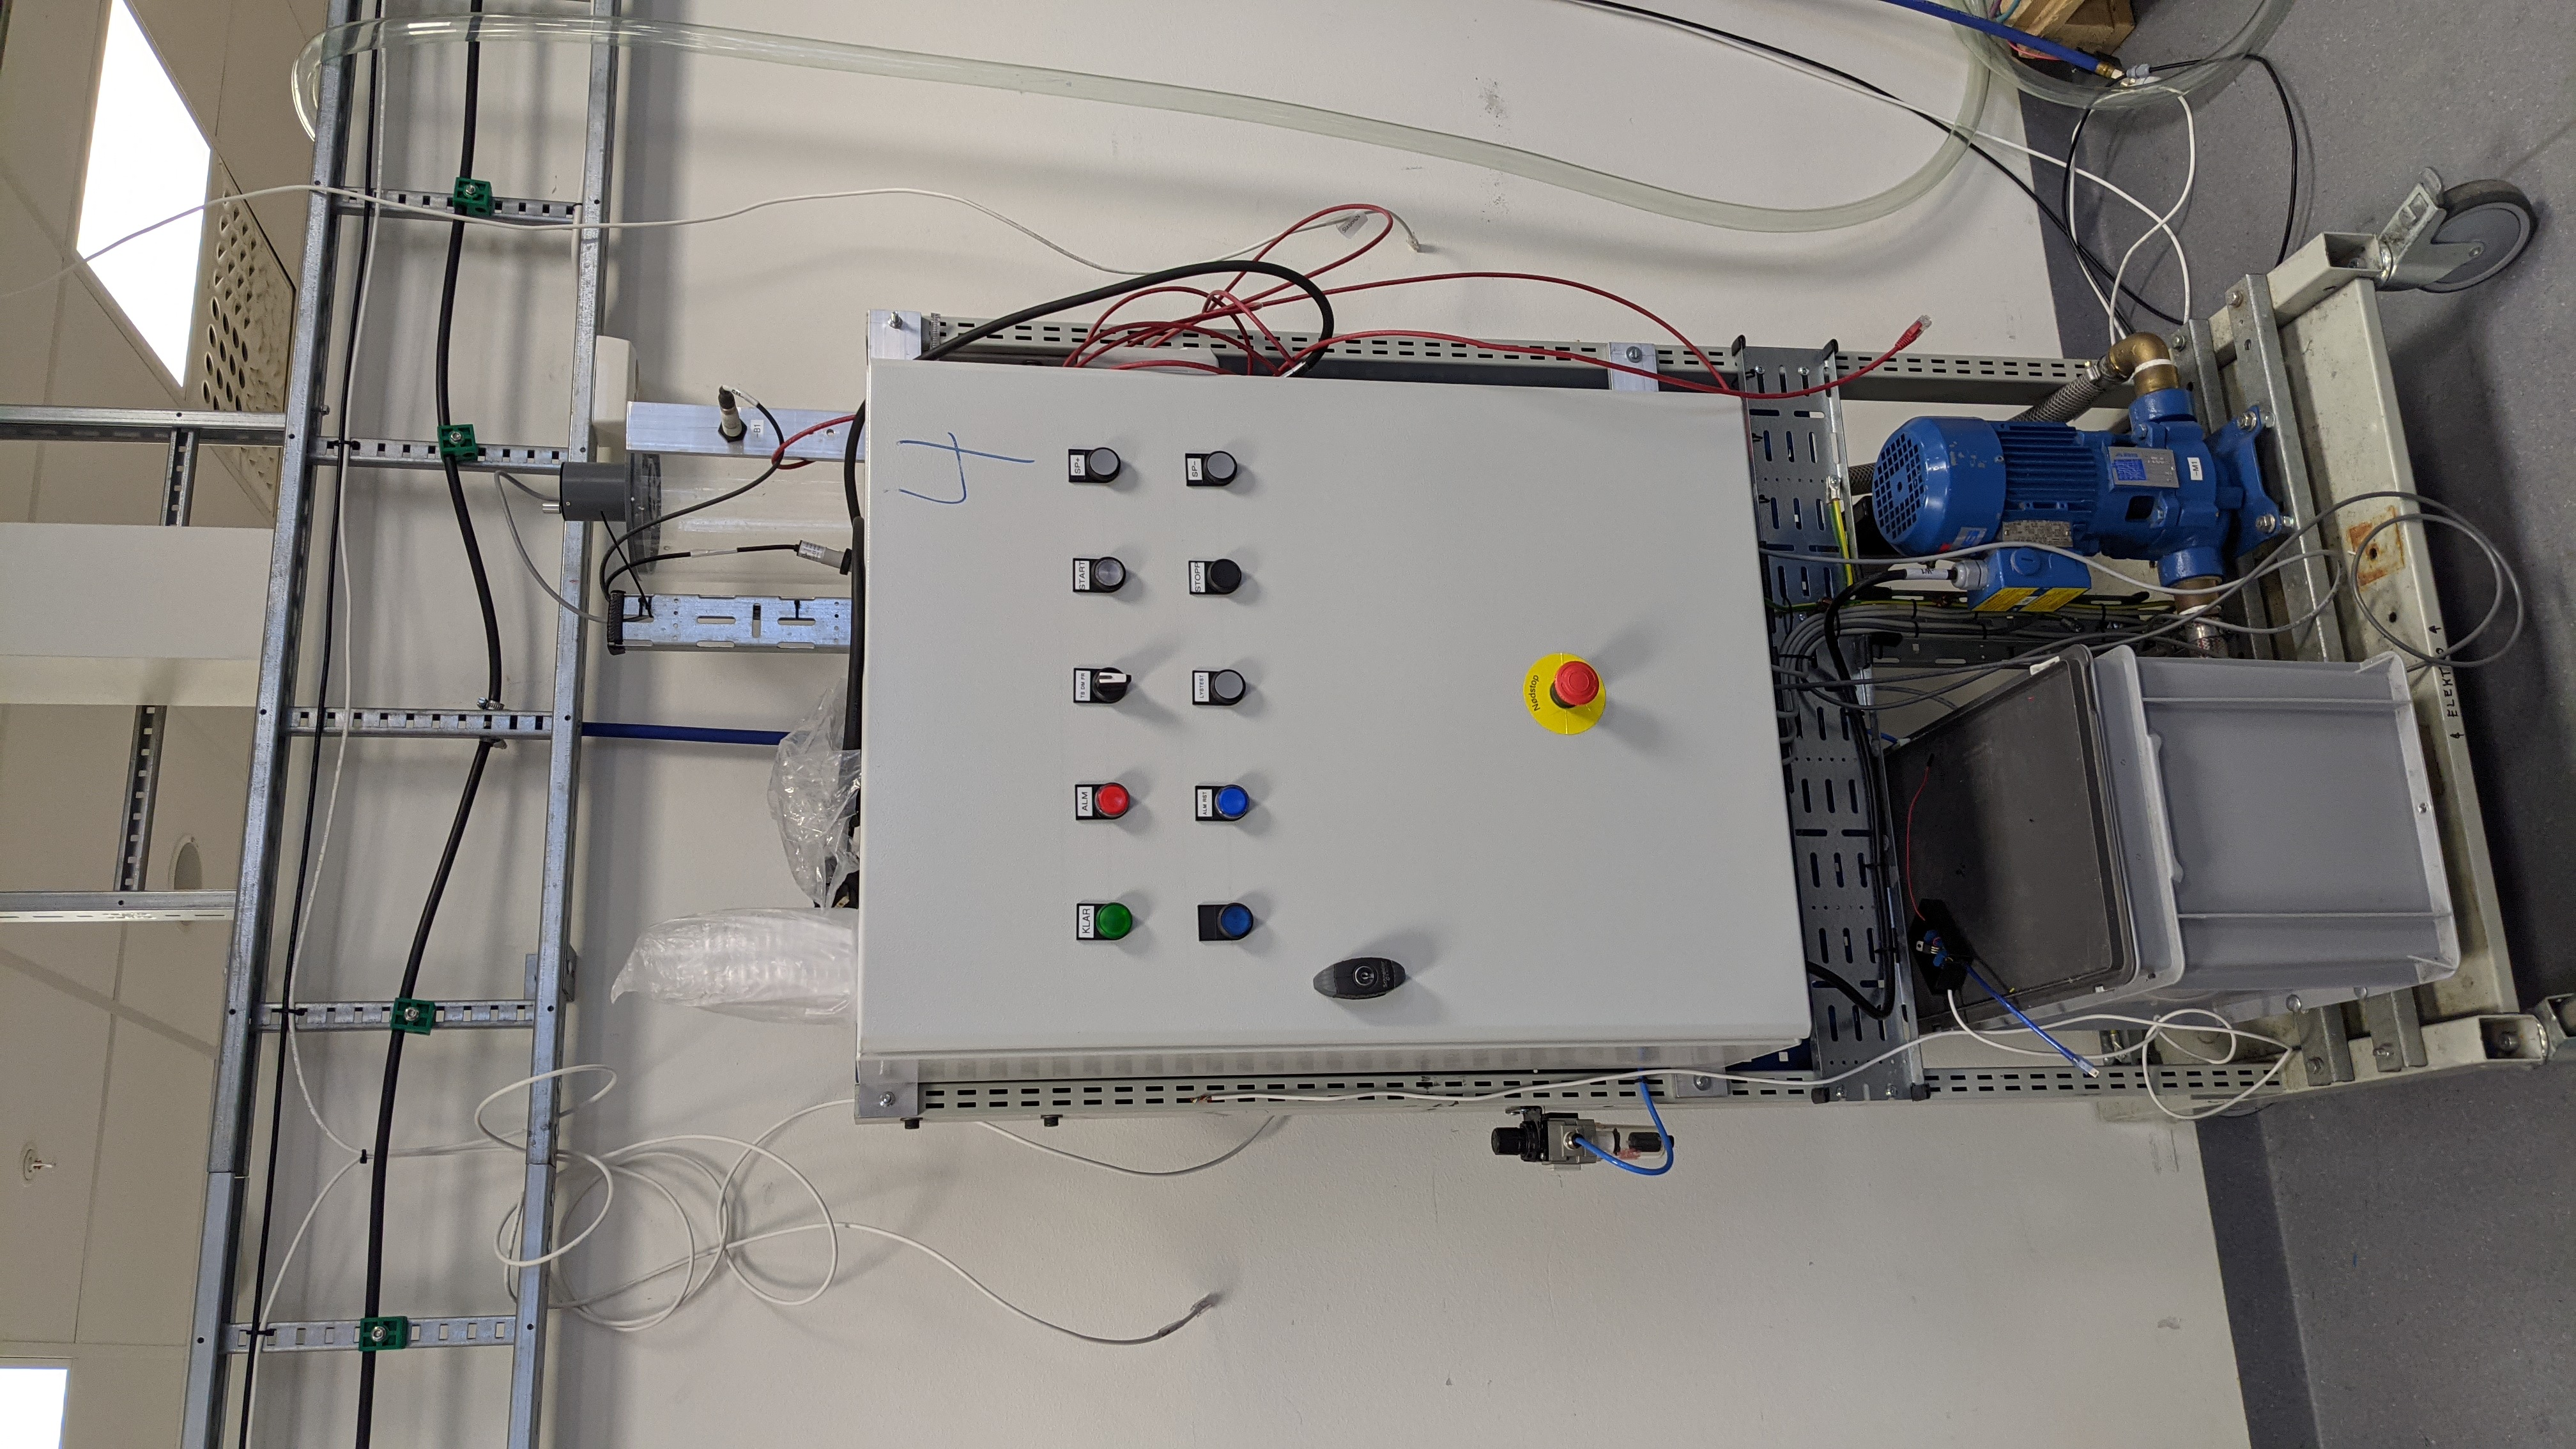
\includegraphics[width=10.5cm,angle=-90]{stasjon04x01.jpg}$$

Stasjon 04 er en Gand reguleringsstasjon. Den er bygget for å kunne øve på uliker typer regulering. På denne stasjonen kan det utføres øvelser med tilbakekoblet regulering (direkte og reverserende), kaskadekoblet regulering og foroverkoblet regulering. 
\section{Stasjon 05}

$$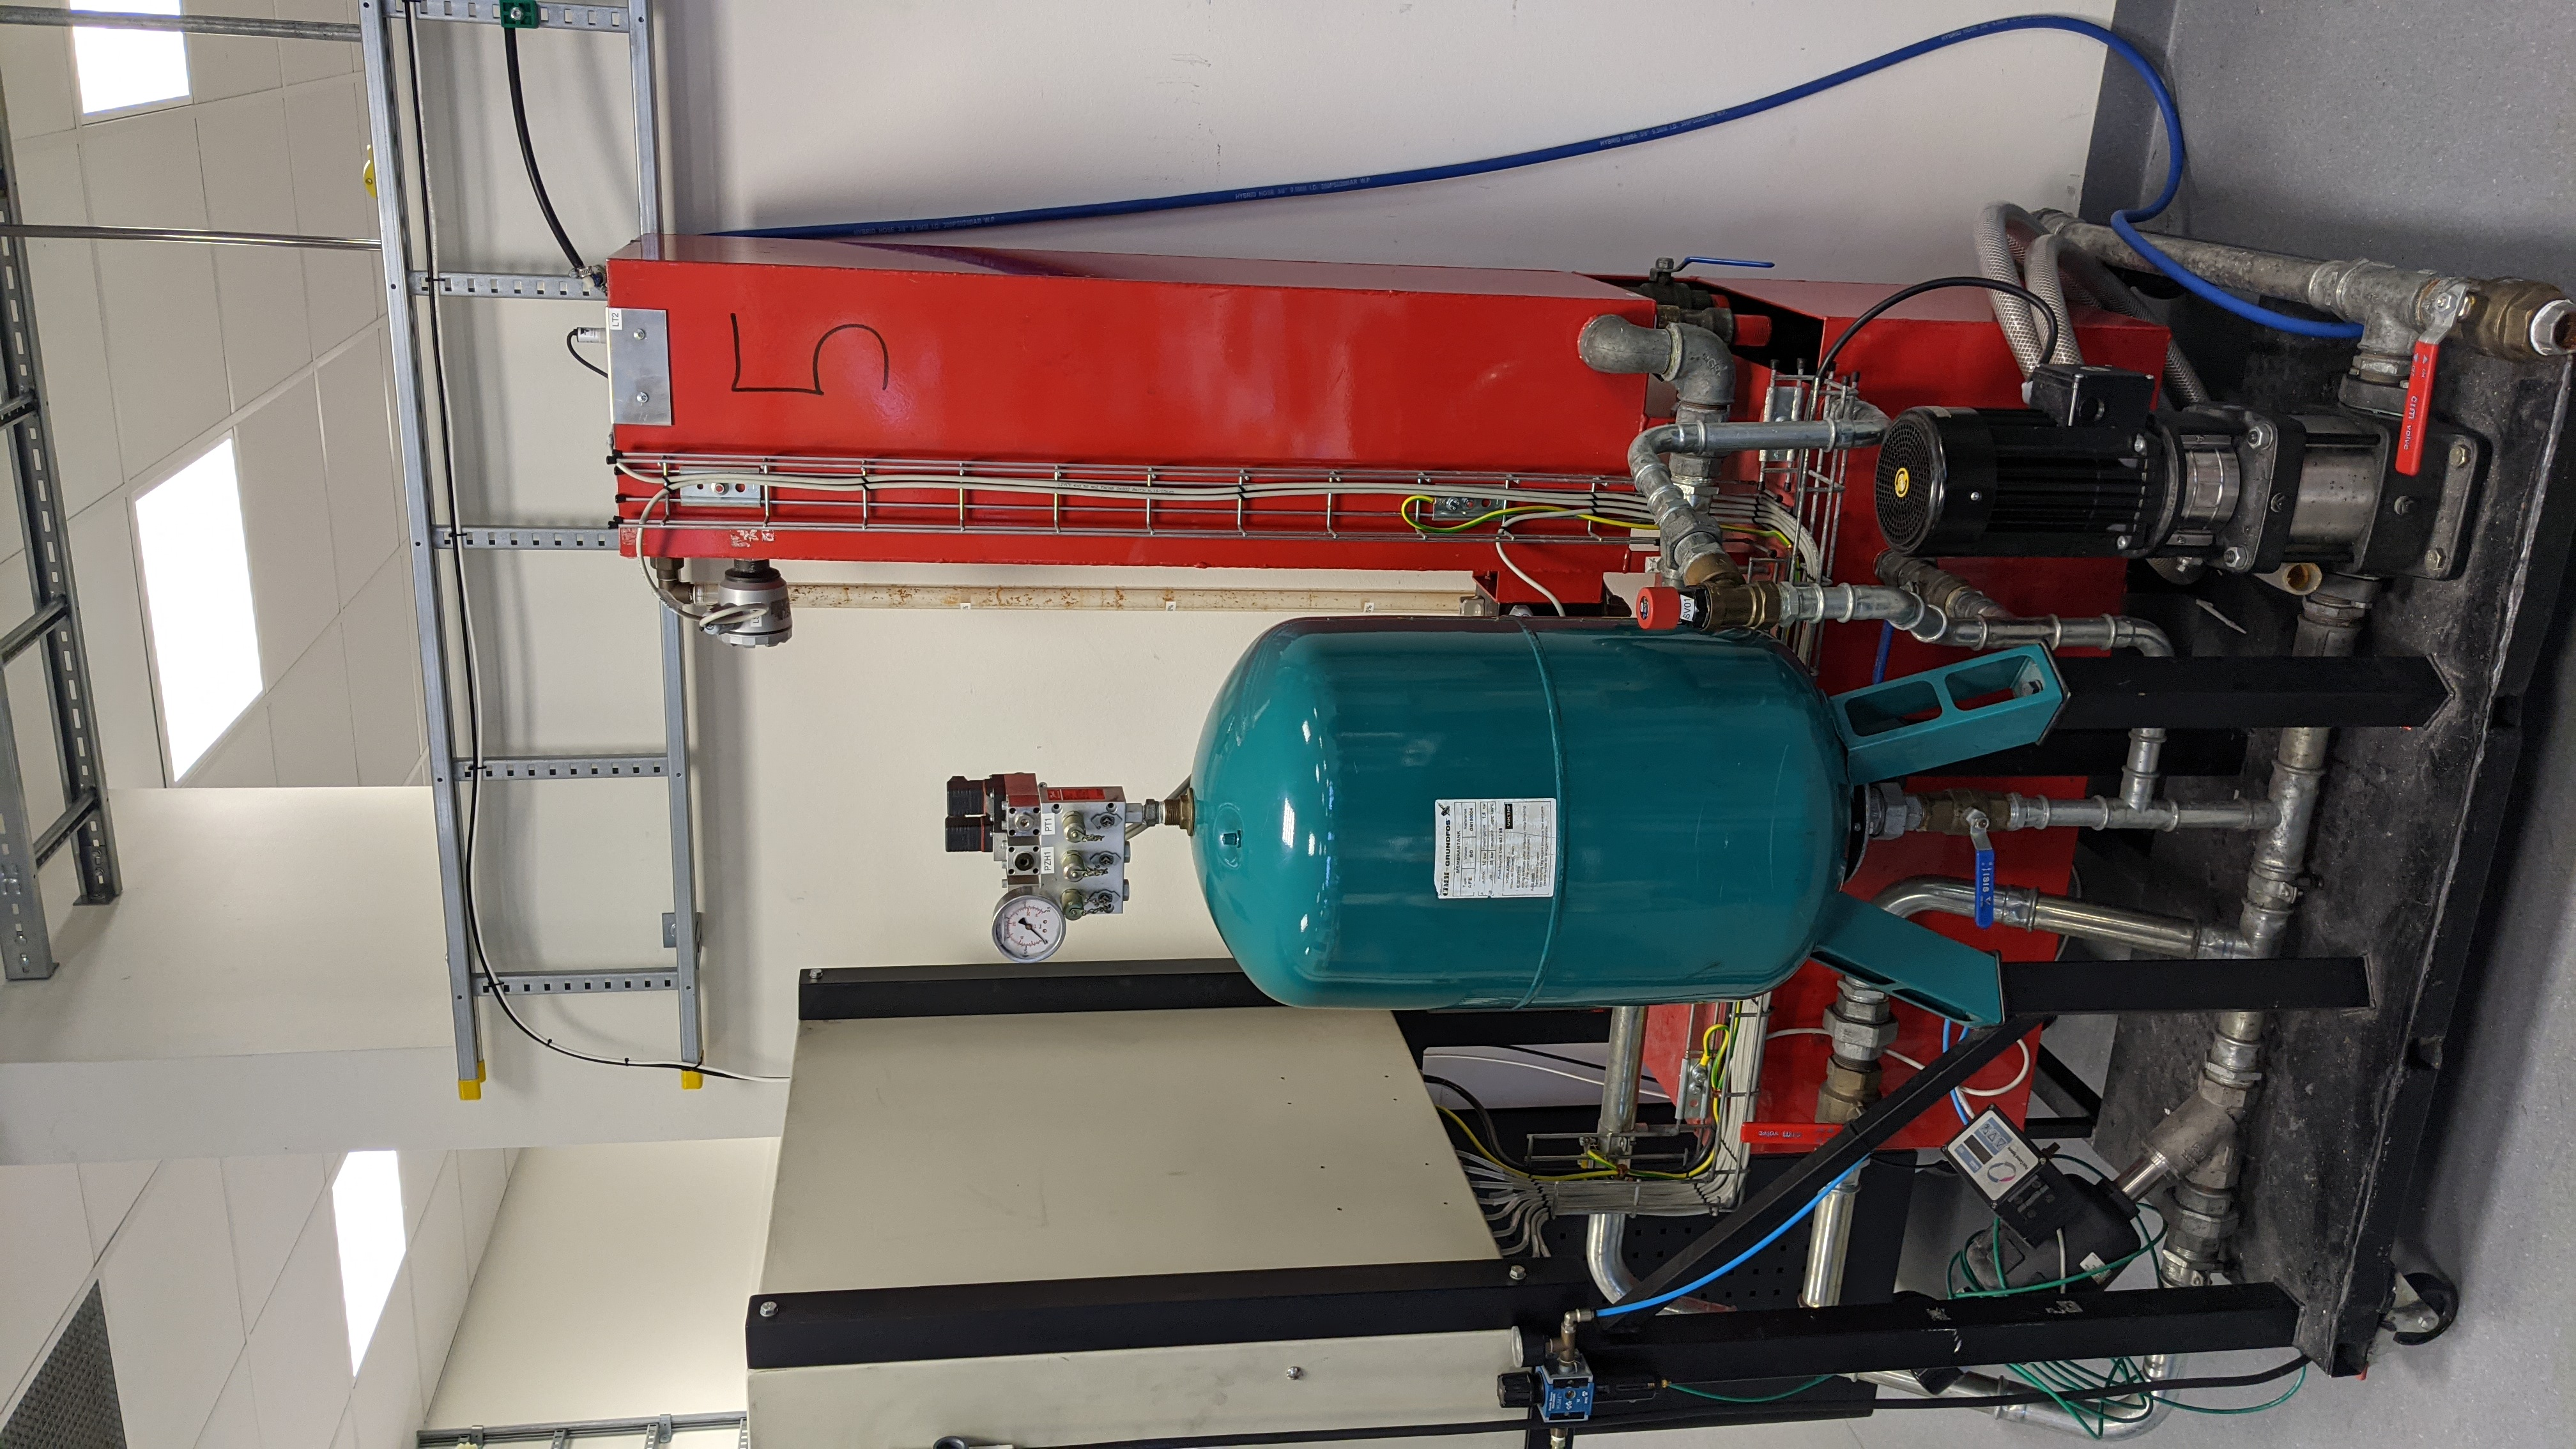
\includegraphics[width=10.5cm,angle=-90]{stasjon05x01.jpg}$$

Stasjon 05 er en reguleringsstasjon gitt til klassen av Kverneland Plogfabrikk. Denne stasjonen er fredig koblet og skal brukes til øvelser i feilsøking. 

\section{Stasjon 06}

$$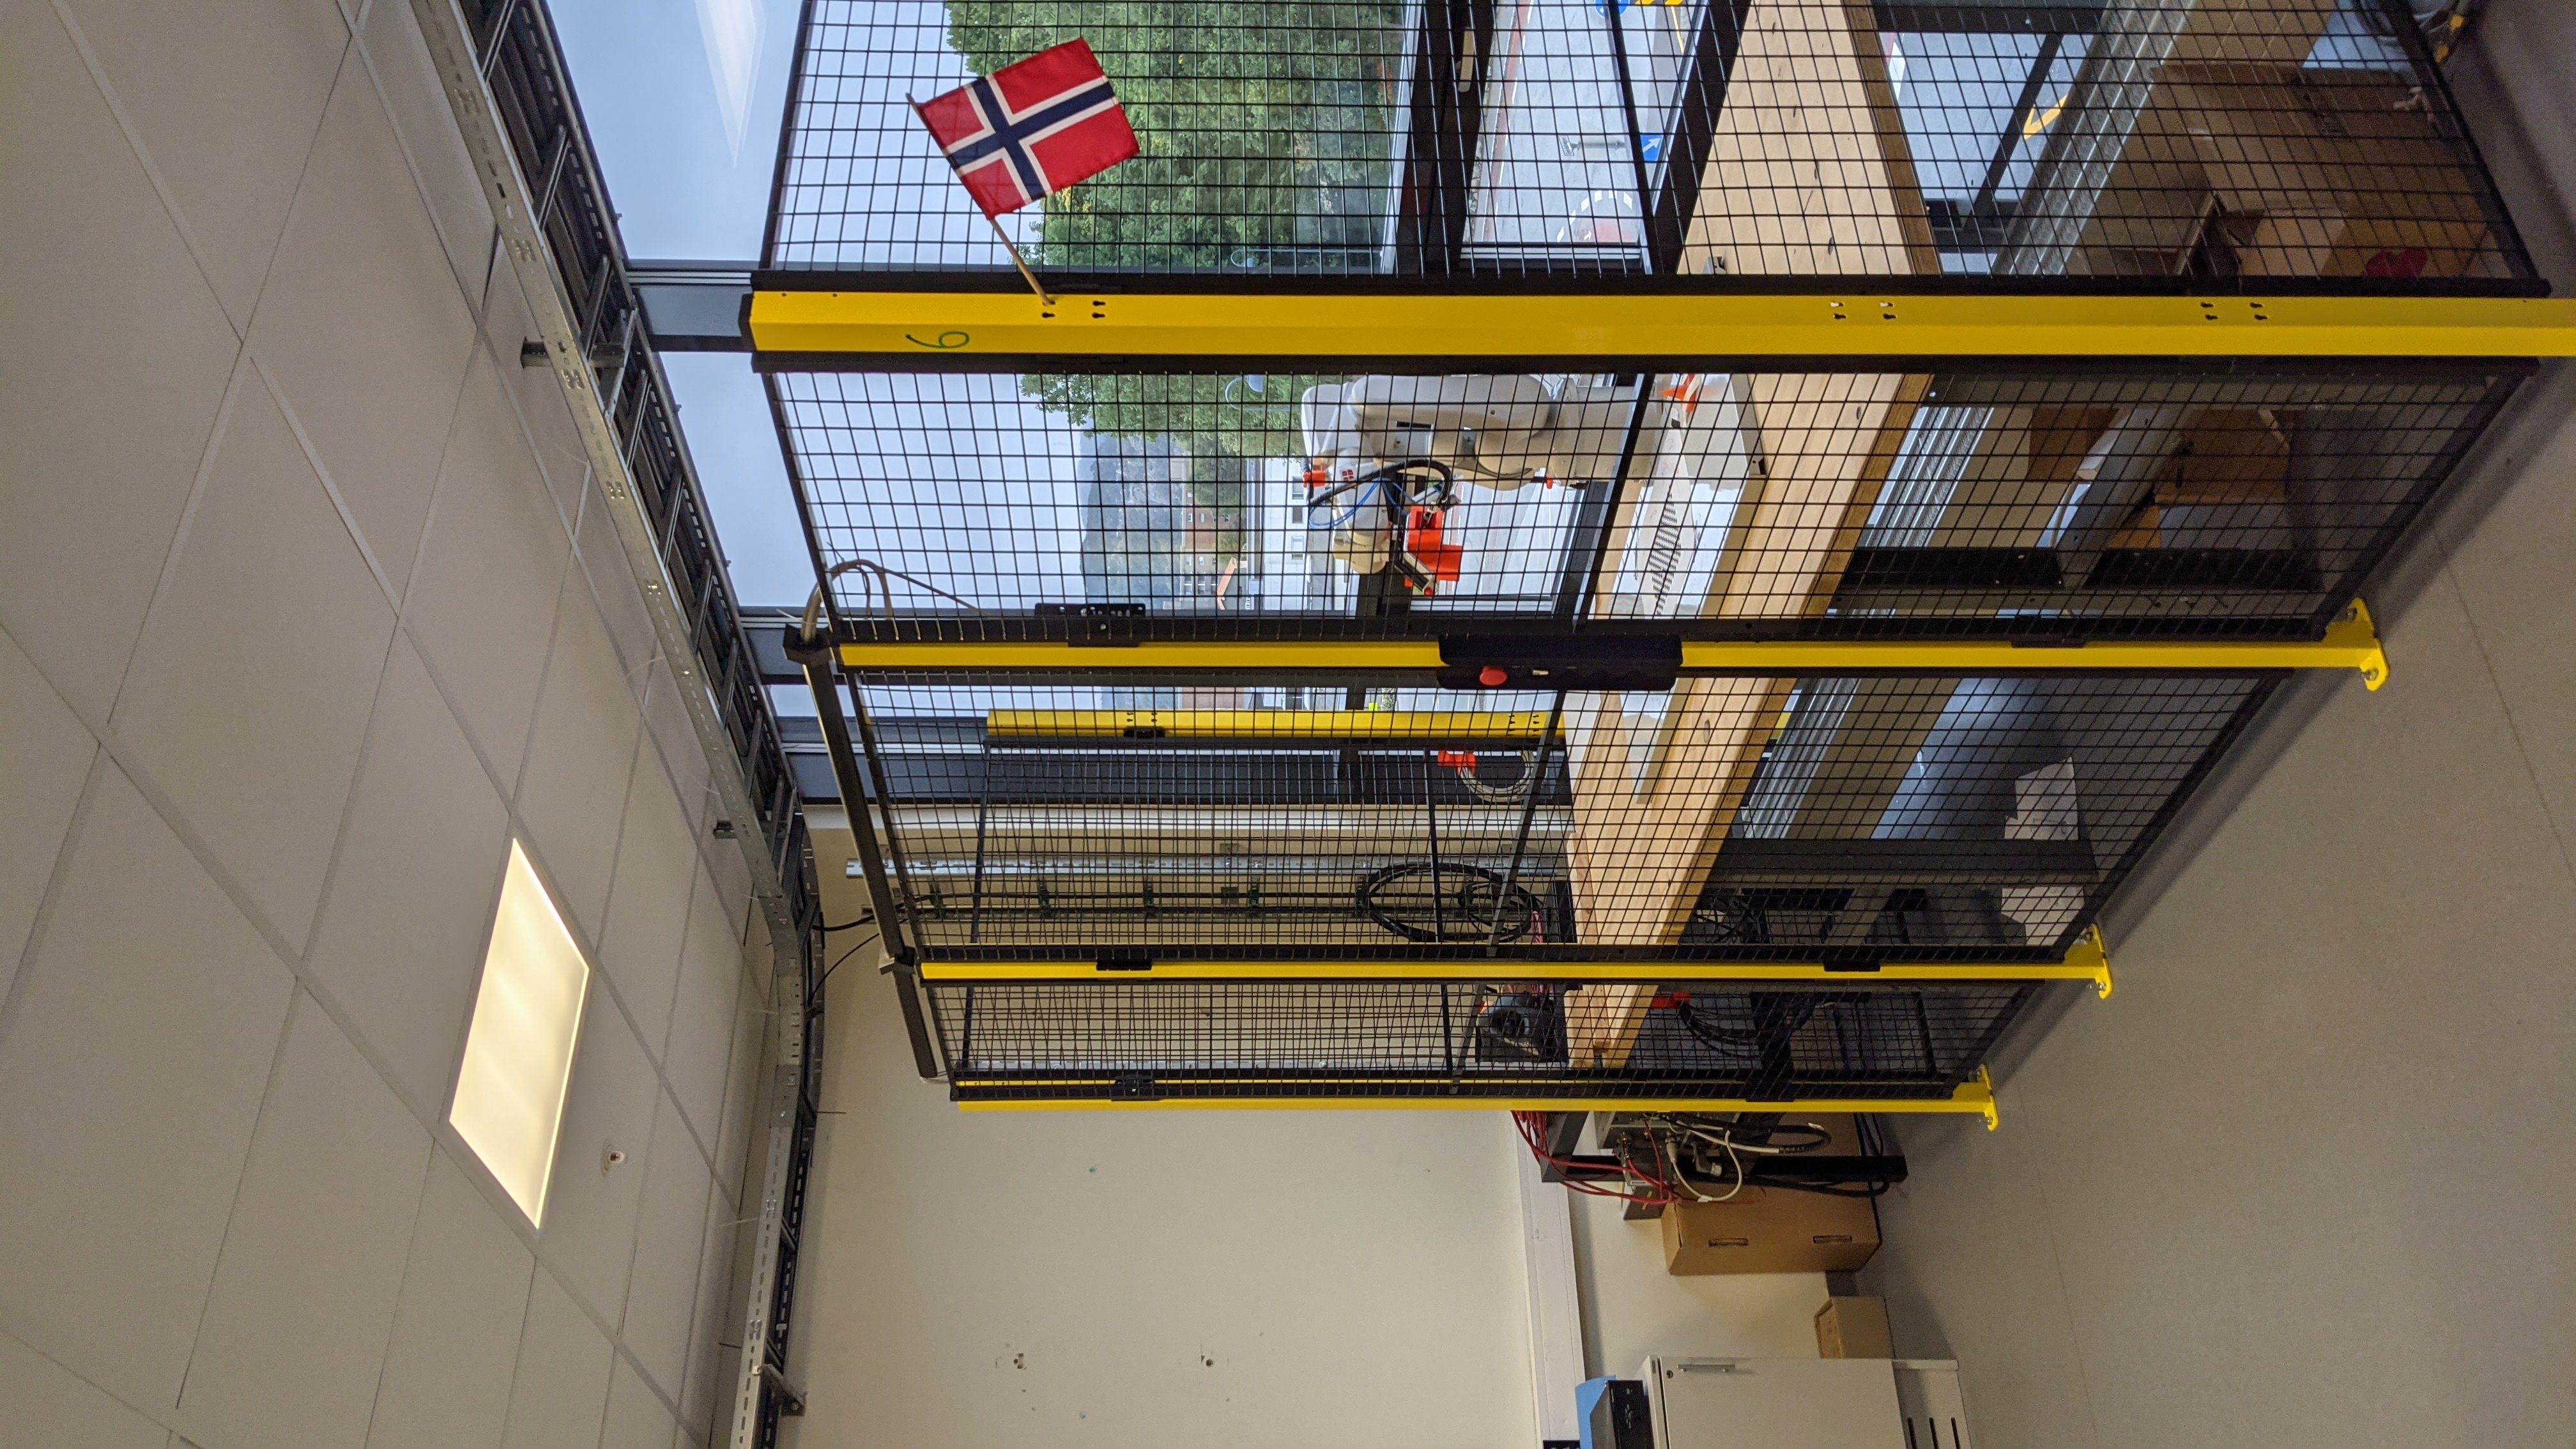
\includegraphics[width=10.5cm,angle=-90]{stasjon06x01.jpg}$$

Stasjon 06 er en robot med sikkerhetsbur. Denne brukes til øvelser i robotprogrammering og robot sikkerhet. 
\section{Stasjon 07}

$$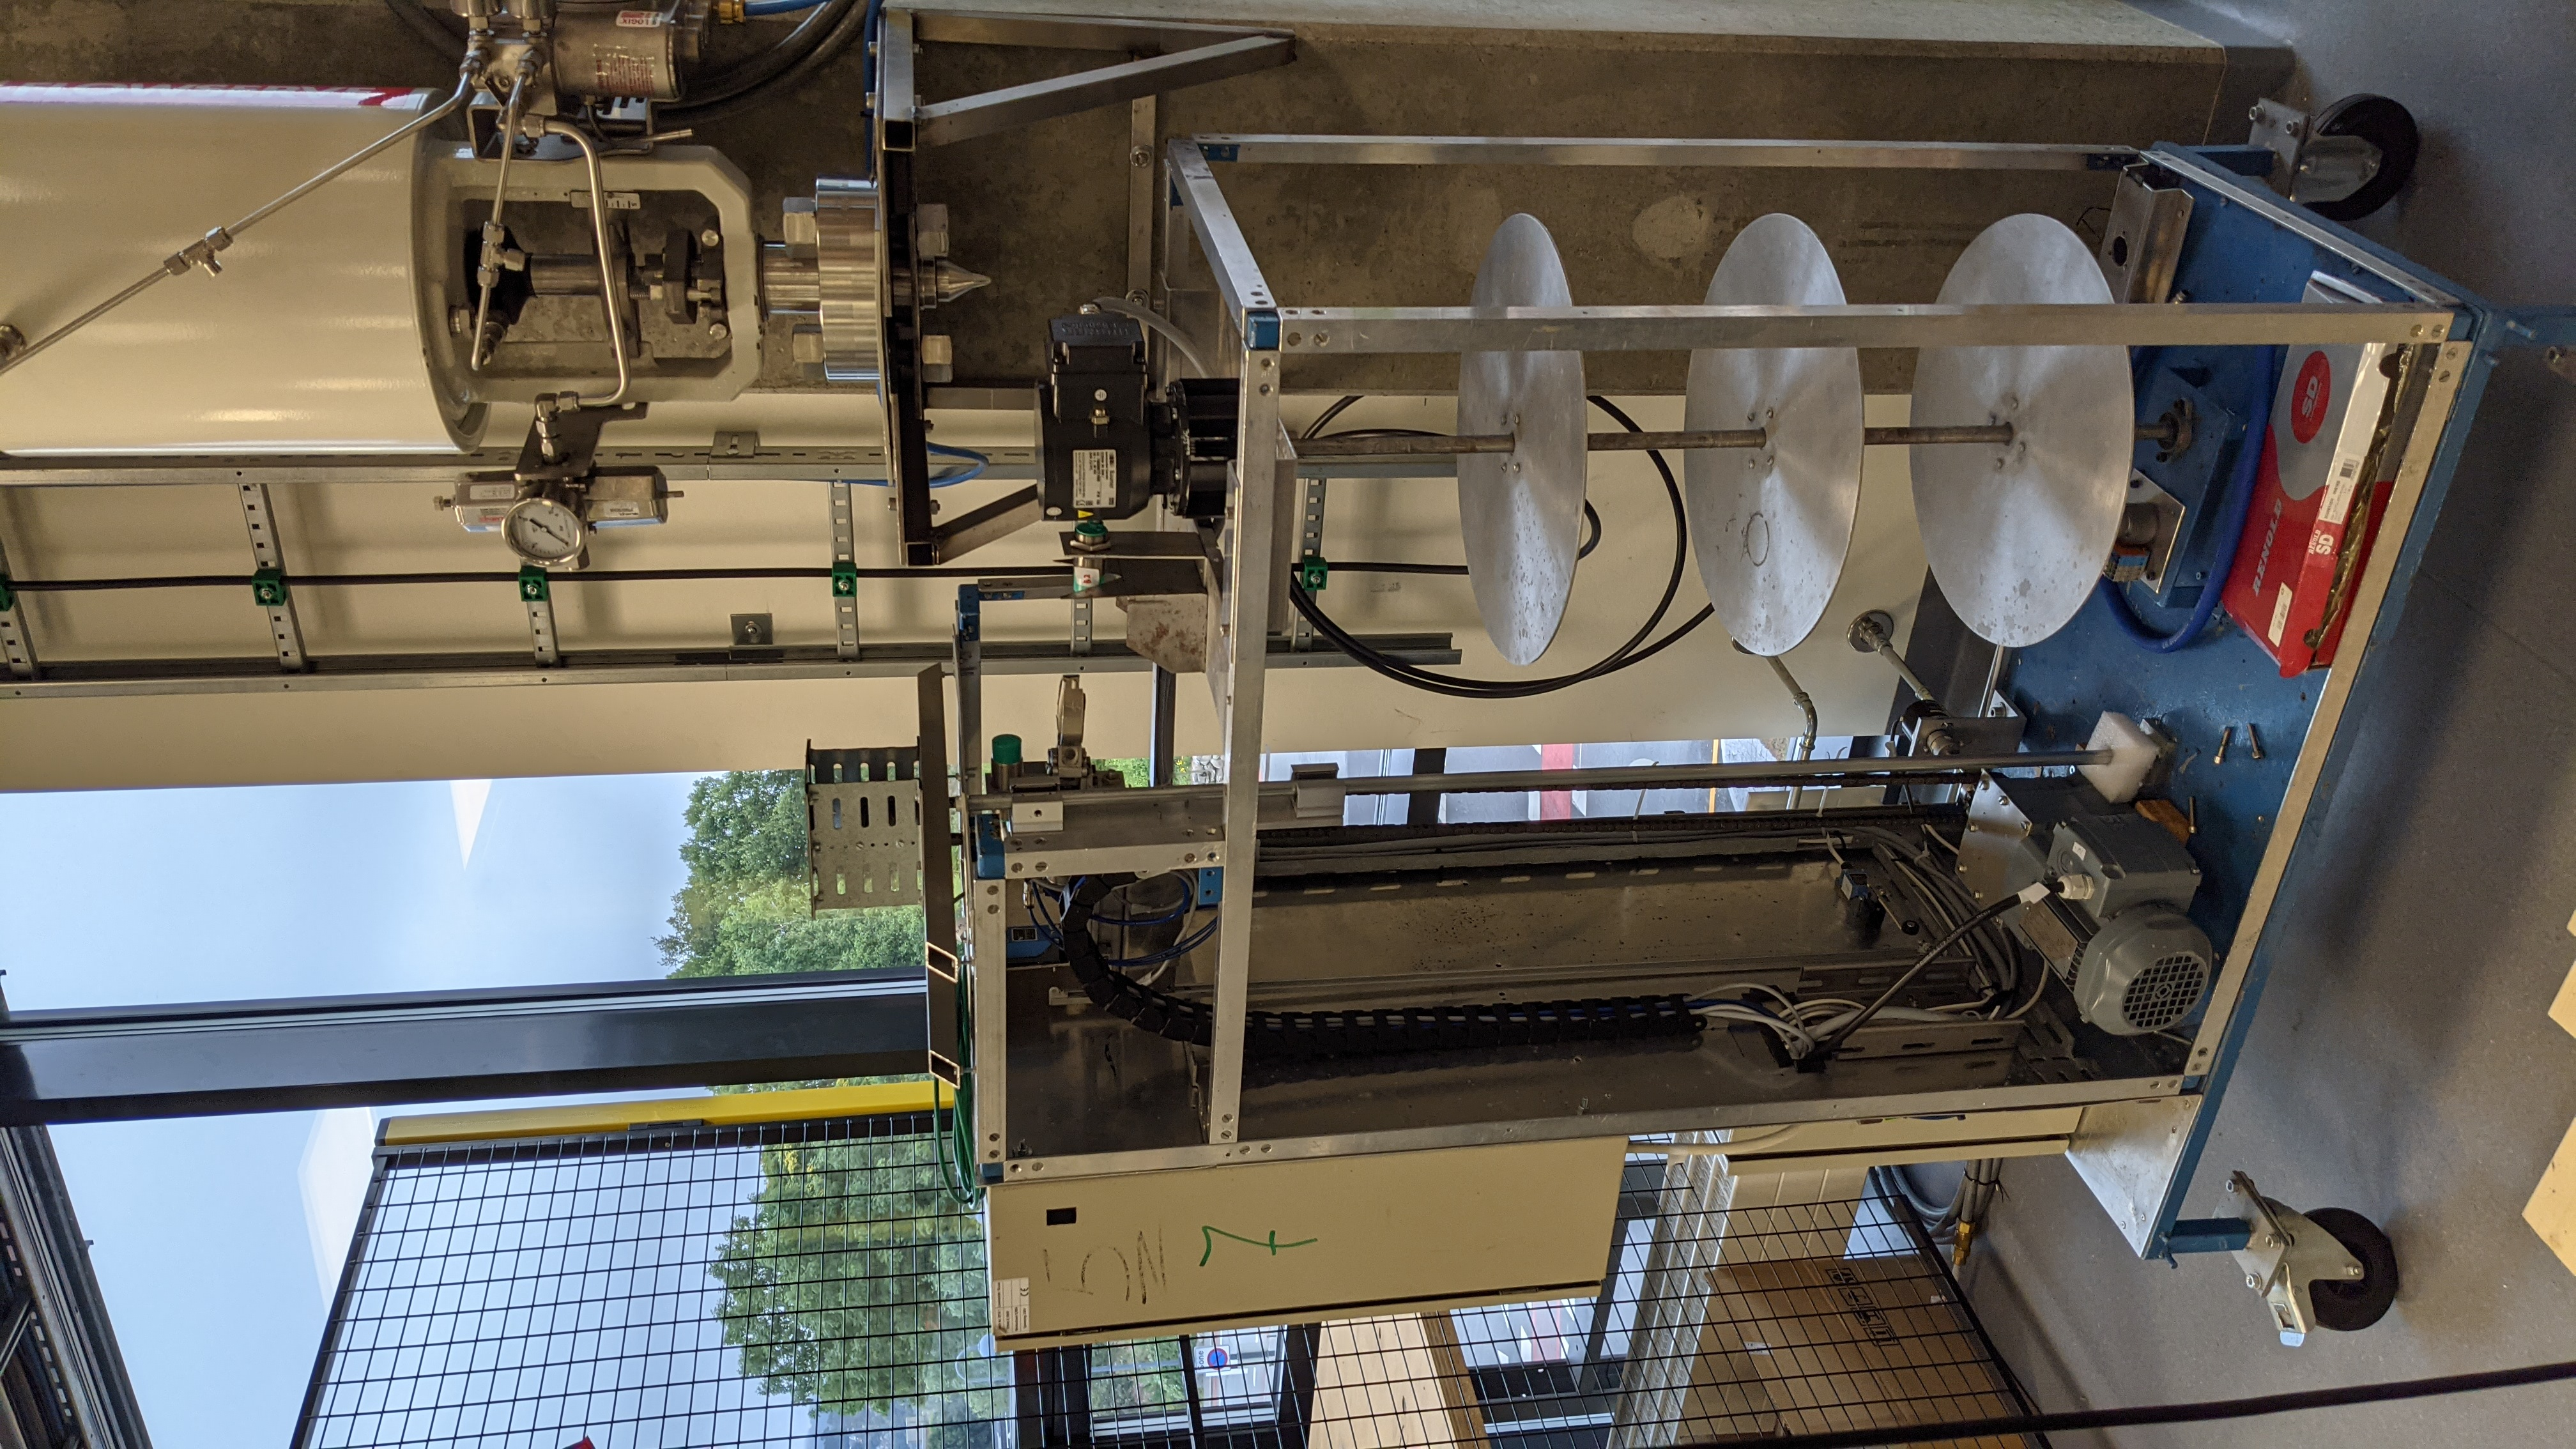
\includegraphics[width=10.5cm,angle=-90]{stasjon07x01.jpg}$$

Stasjon 7 er en brusautomat eller autobar. Denne er under oppbyggning og oppgaver på den vil gå ut på å gjøre den ferdig. 




\section{Stasjon 8}

$$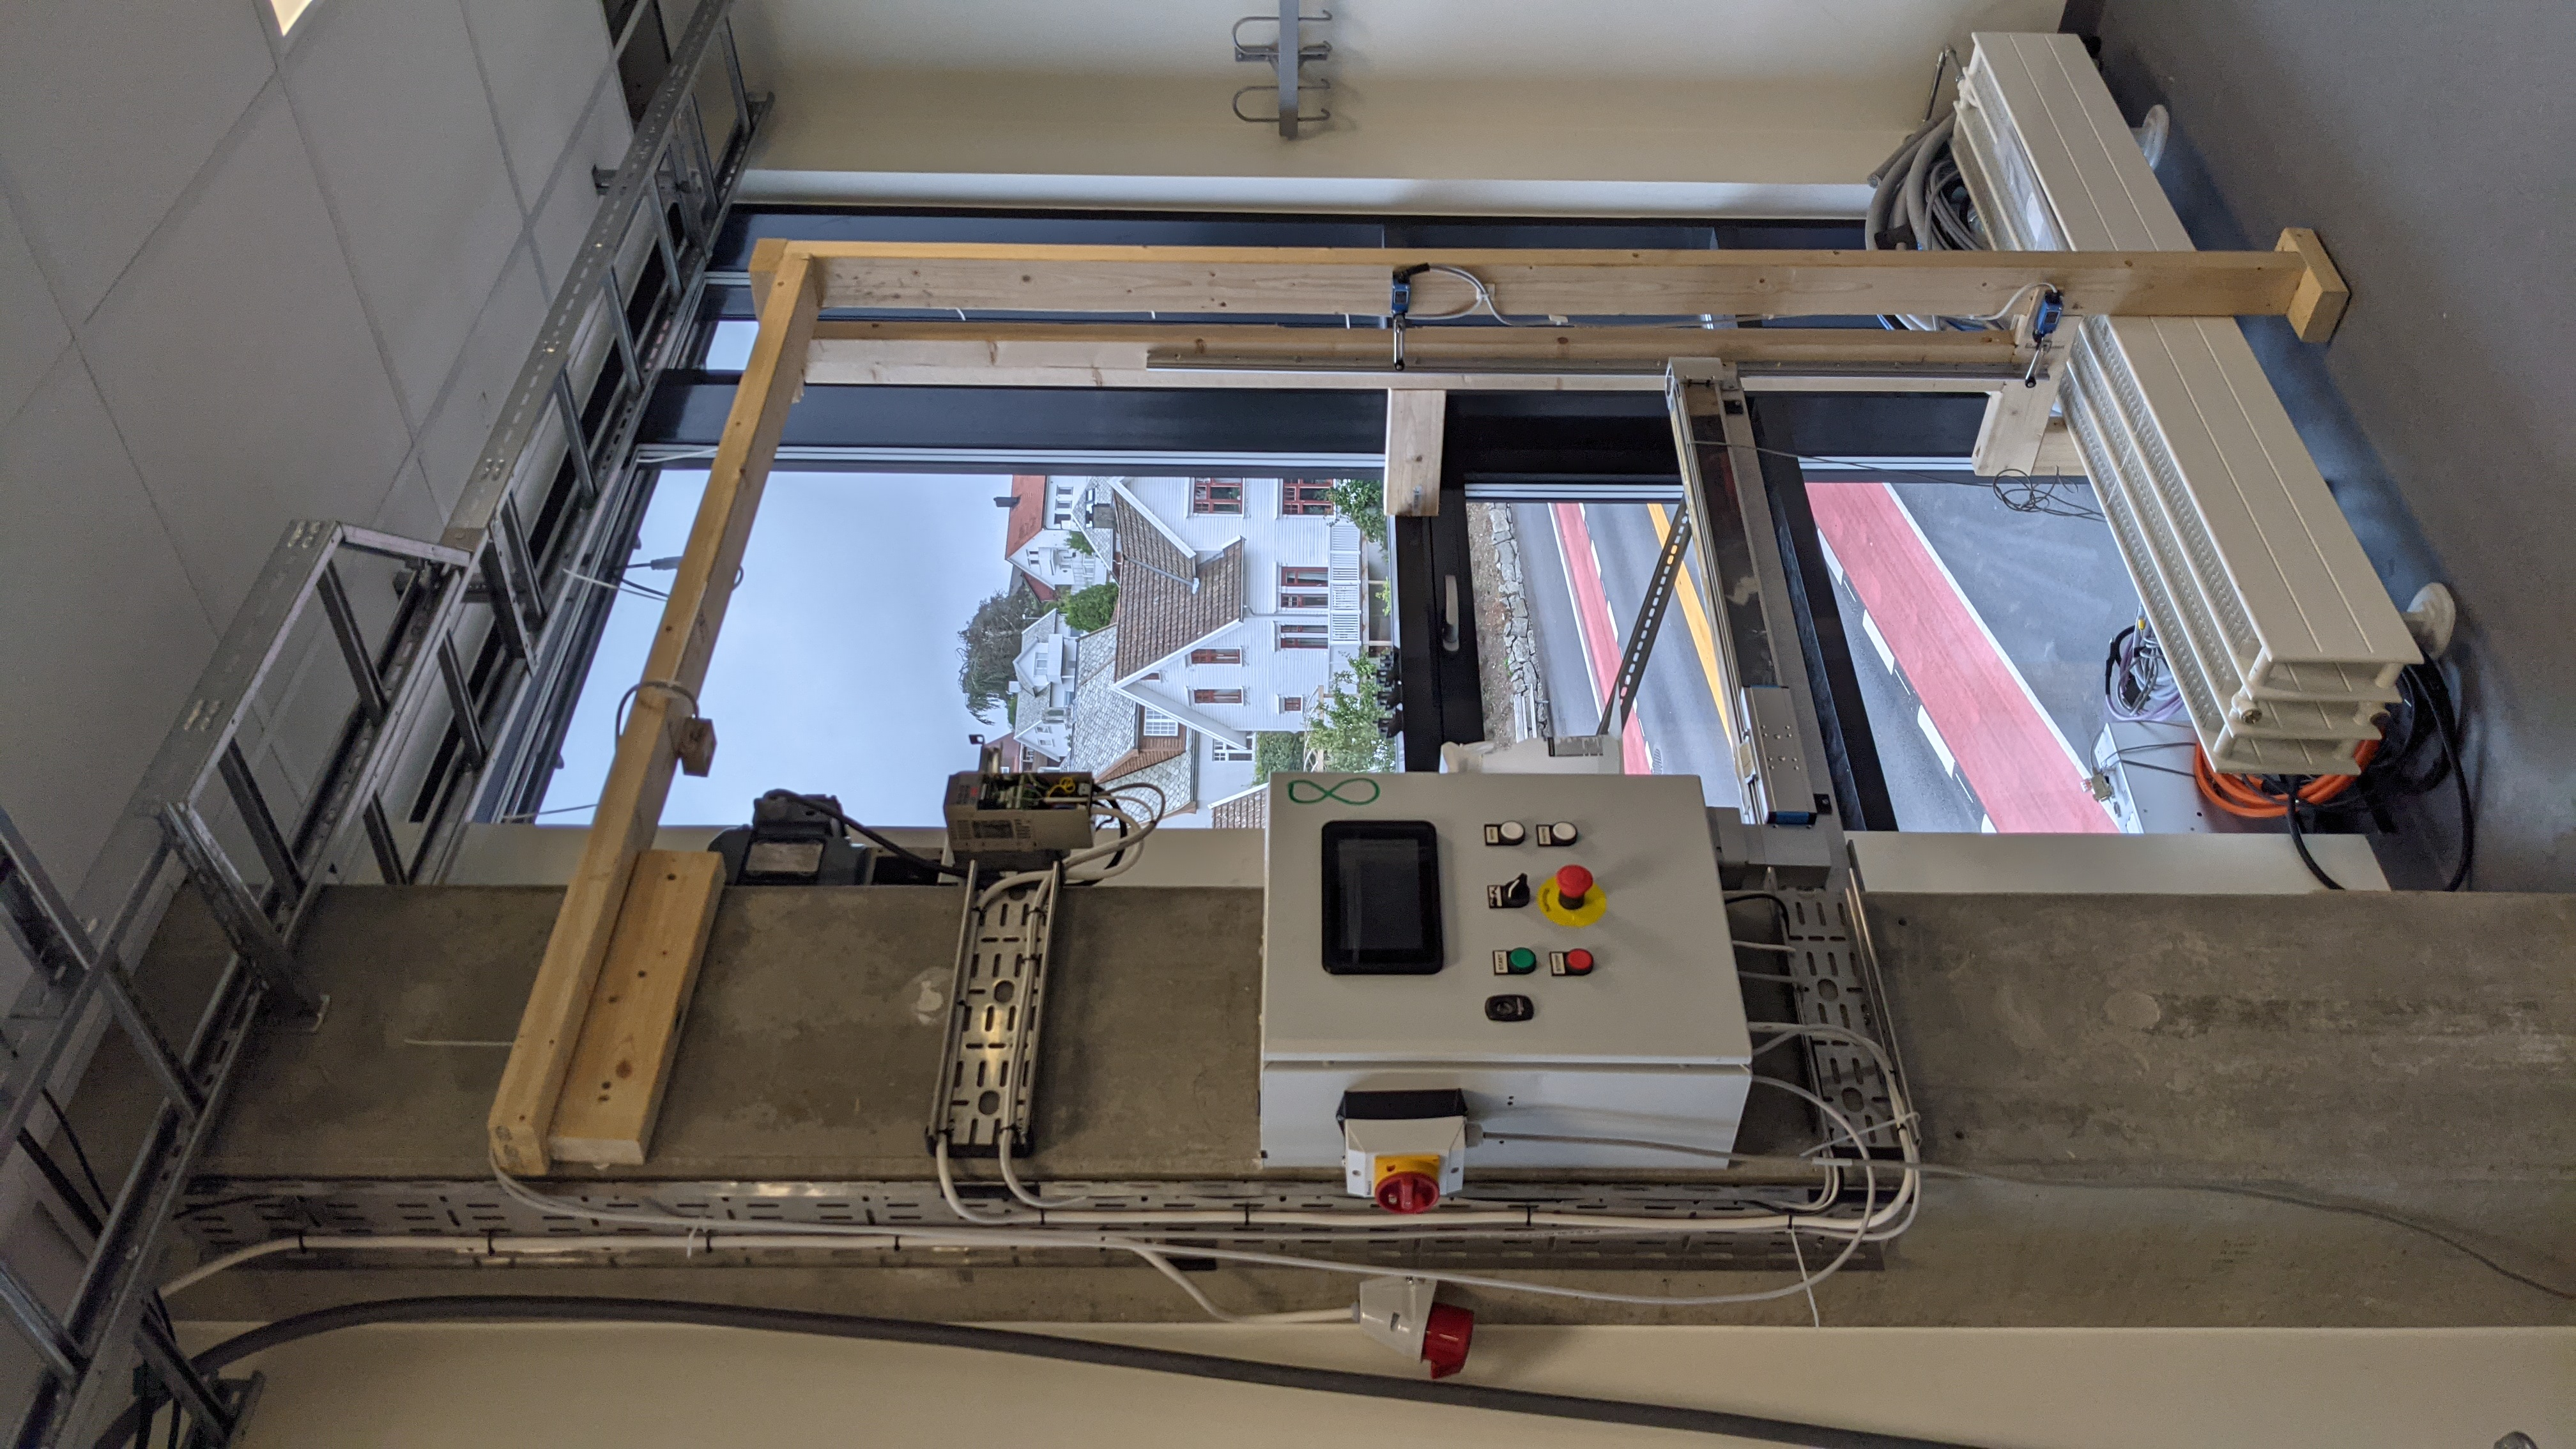
\includegraphics[width=10.5cm,angle=-90]{stasjon08x01.jpg}$$

Stasjon 08 er et XY Aksesystem  for posisjonsregulering med frekvensomformer og servo drive. Denne er også under oppbyggning. 

\section{Stasjon 09}

$$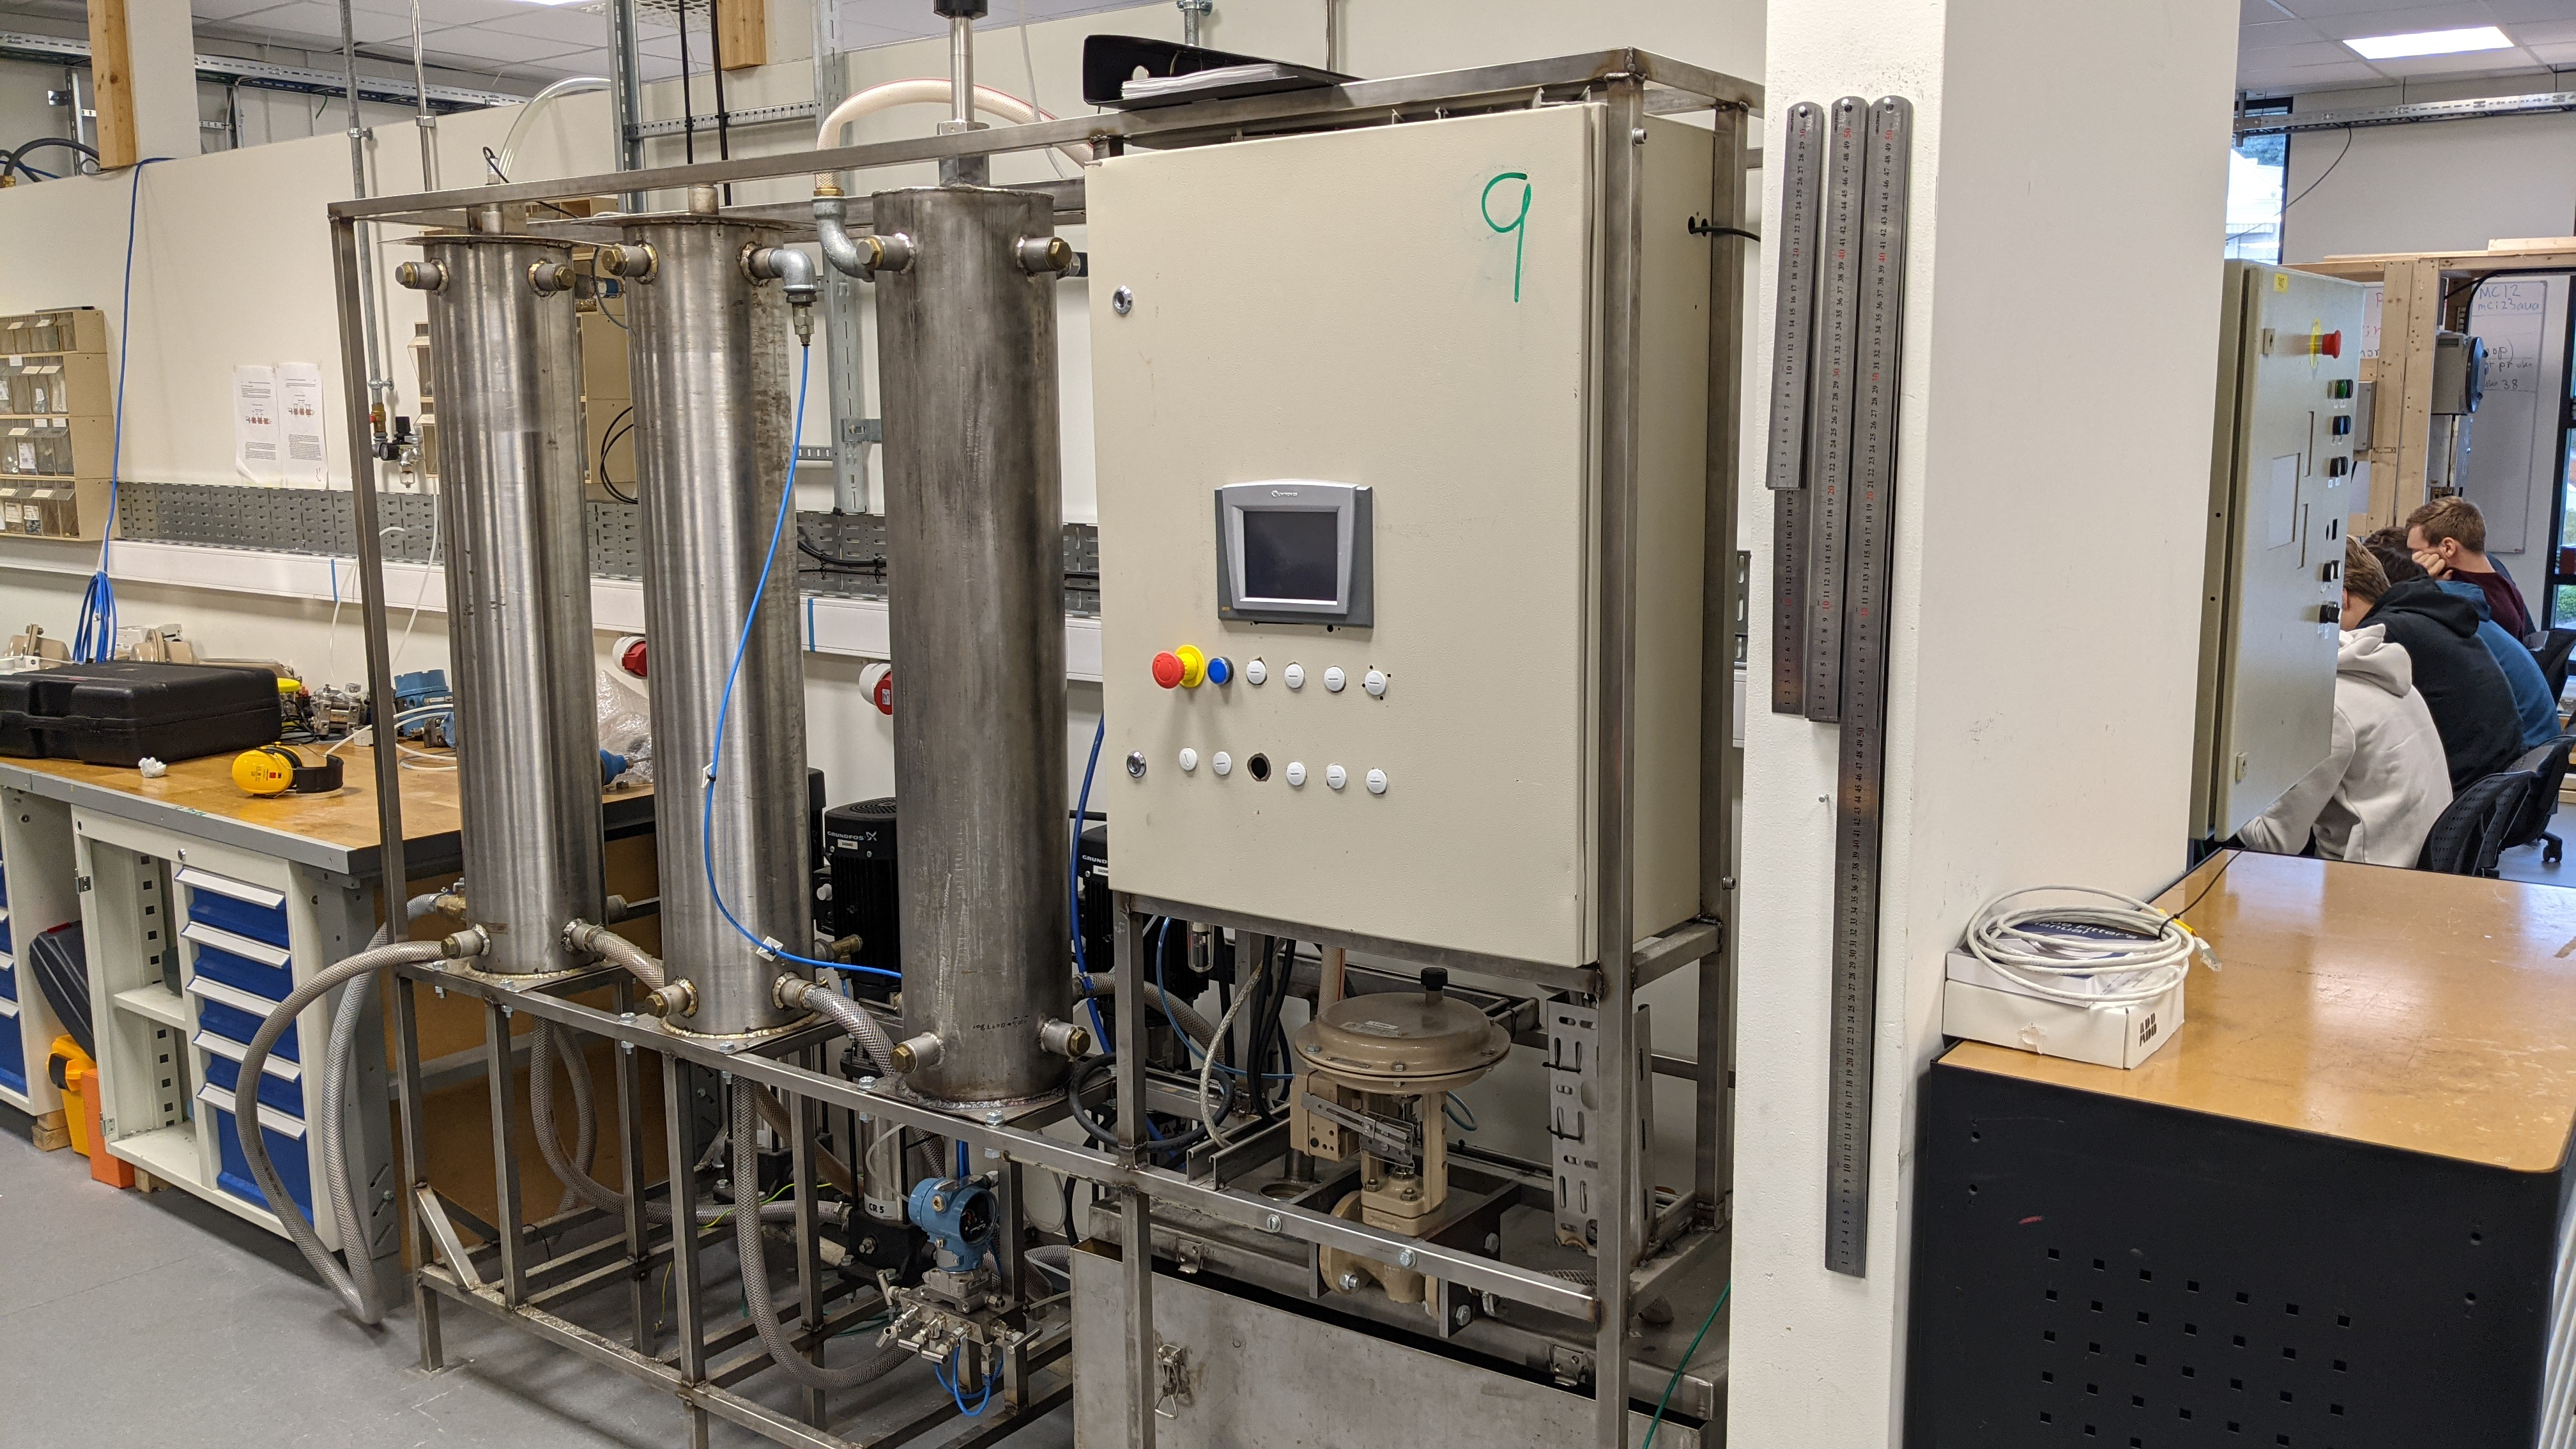
\includegraphics[width=10.5cm]{stasjon09x01.jpg}$$

Stasjon 09 eller de tre tanker er en litt større reguleringsstasjon der vannet pumpes fra  et resovoar og gjennom tre tanker før det sleppes tilbake til resovoaret. Her kan en gjøre øvelser med HMI bygging, innstilling av regulatorene og øvelser på ulike nivåmålesystem. 

\section{Stasjon 10}

$$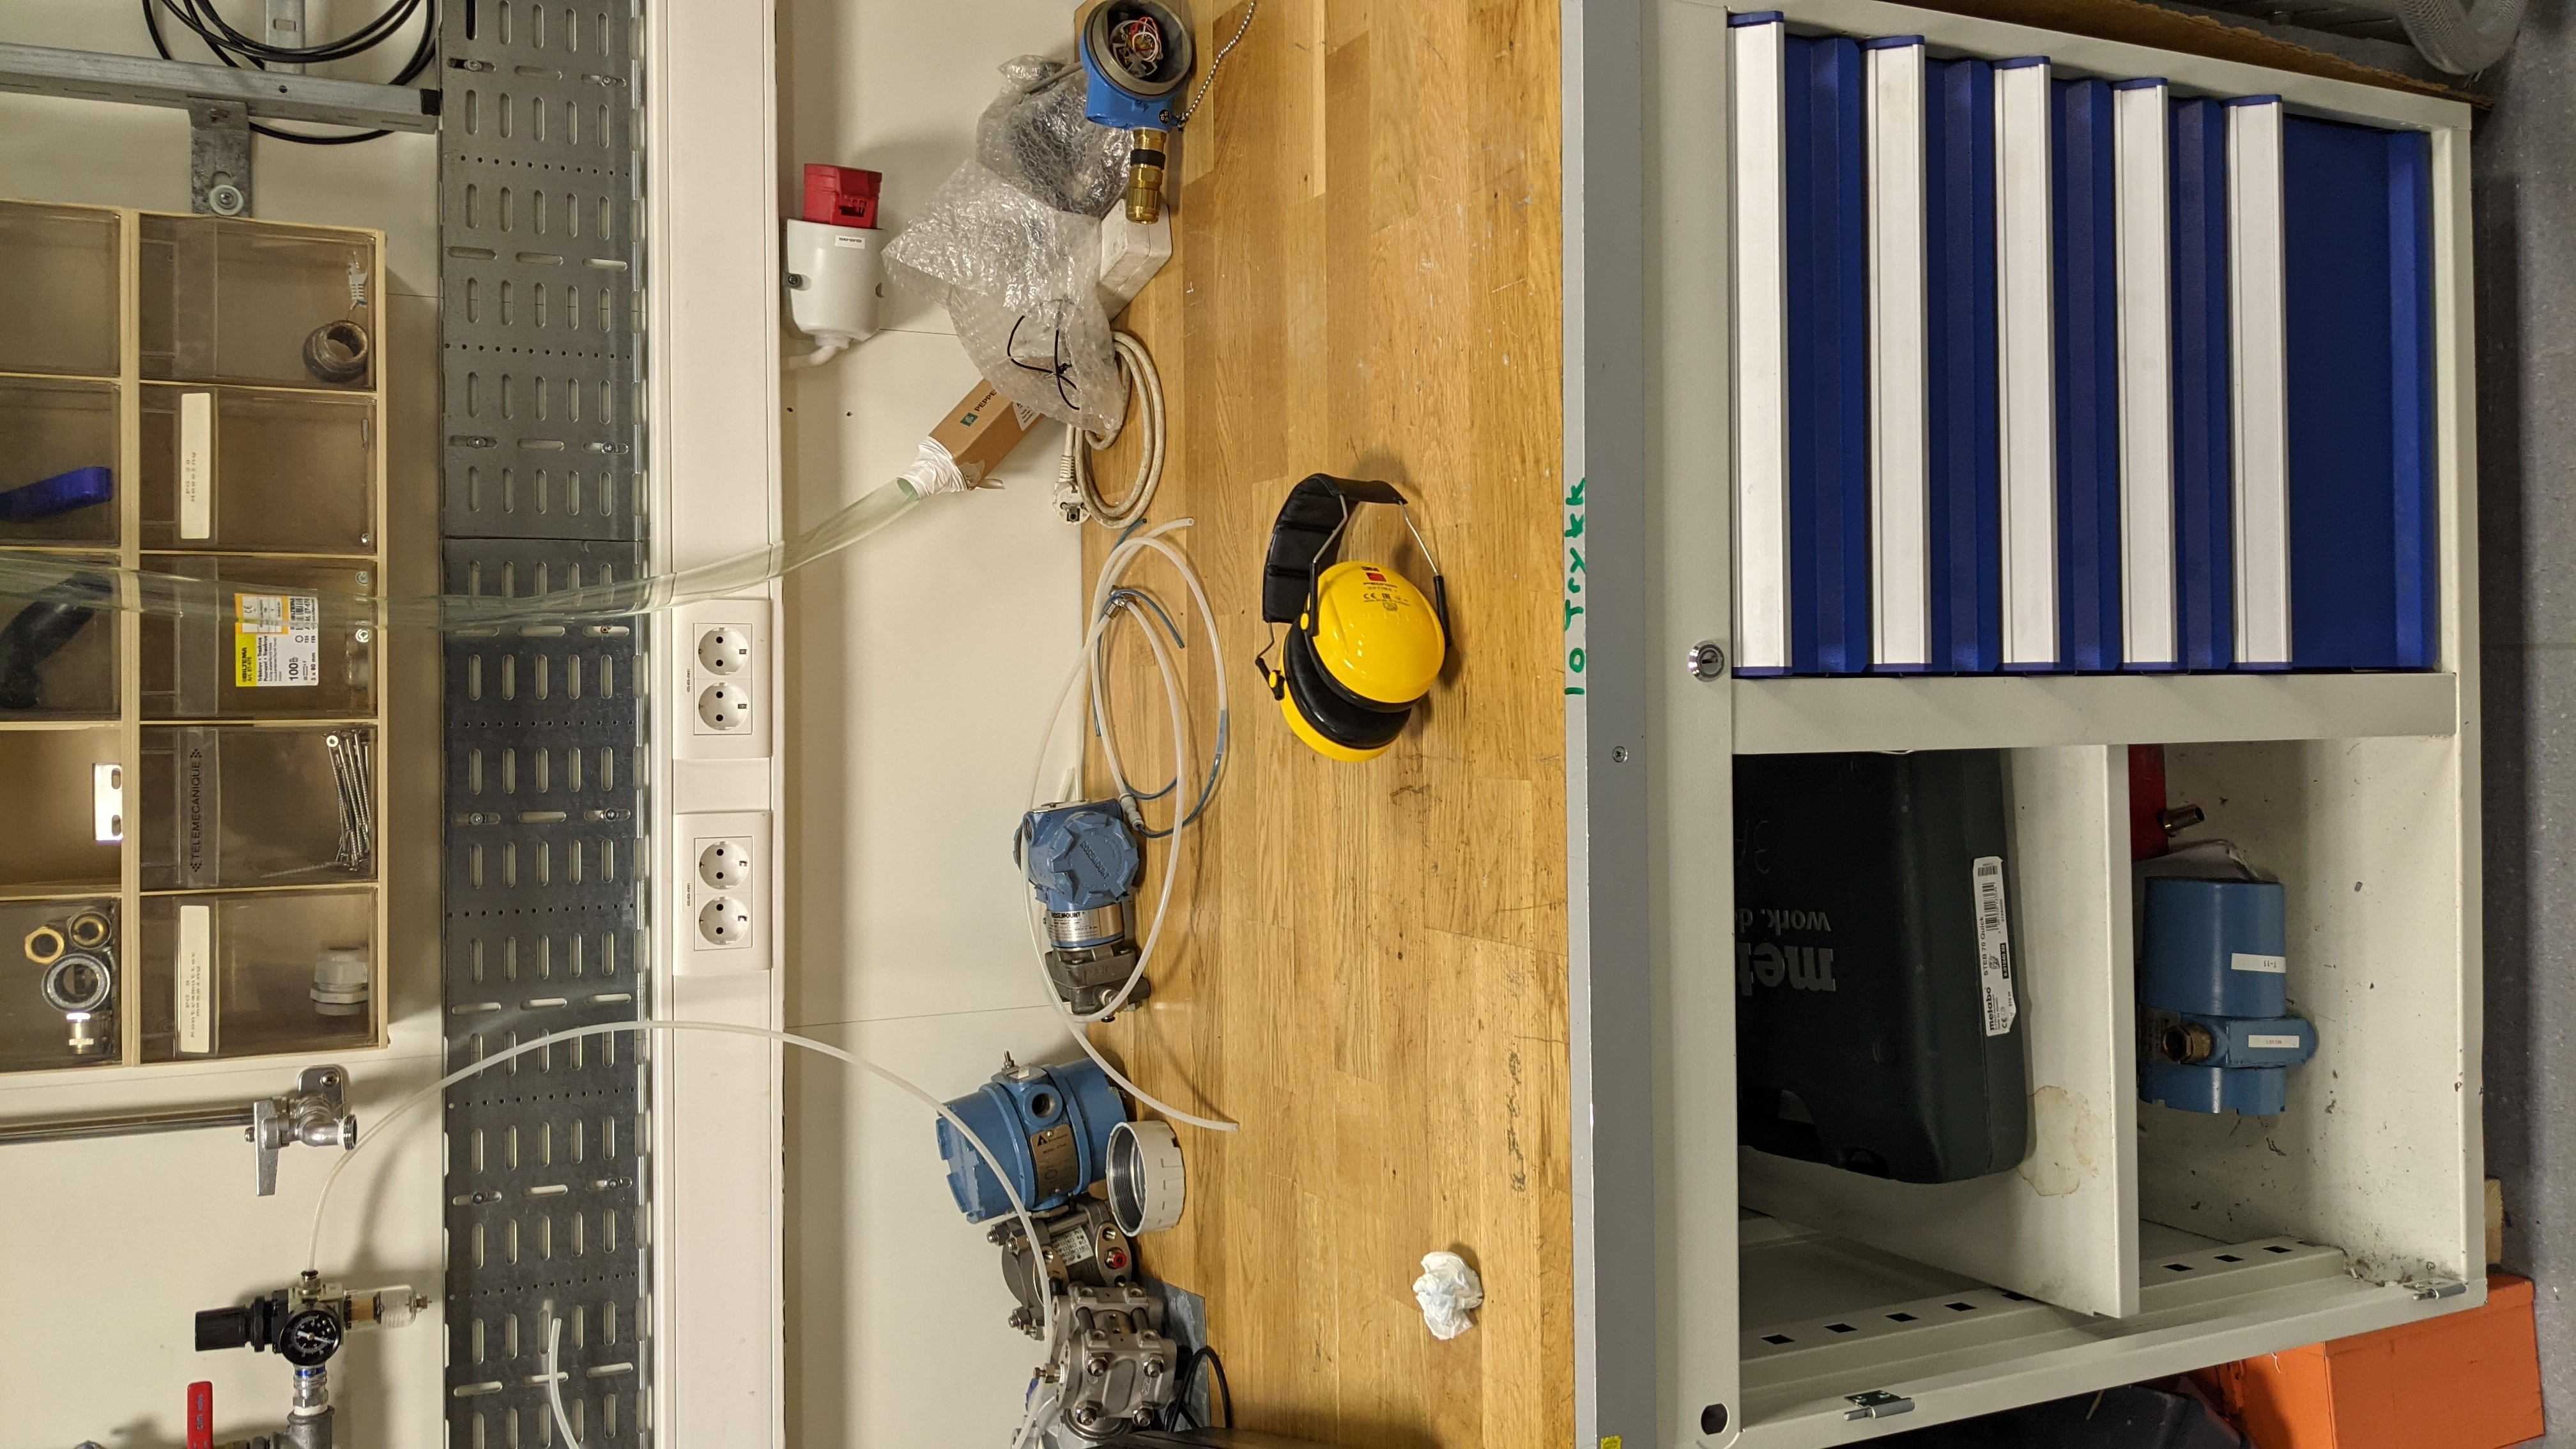
\includegraphics[width=10.5cm,angle=-90]{stasjon10x01.jpg}$$

Stasjon 10 er for benkkalibrering av trykksensorer. 
\section{Stasjon 11}

$$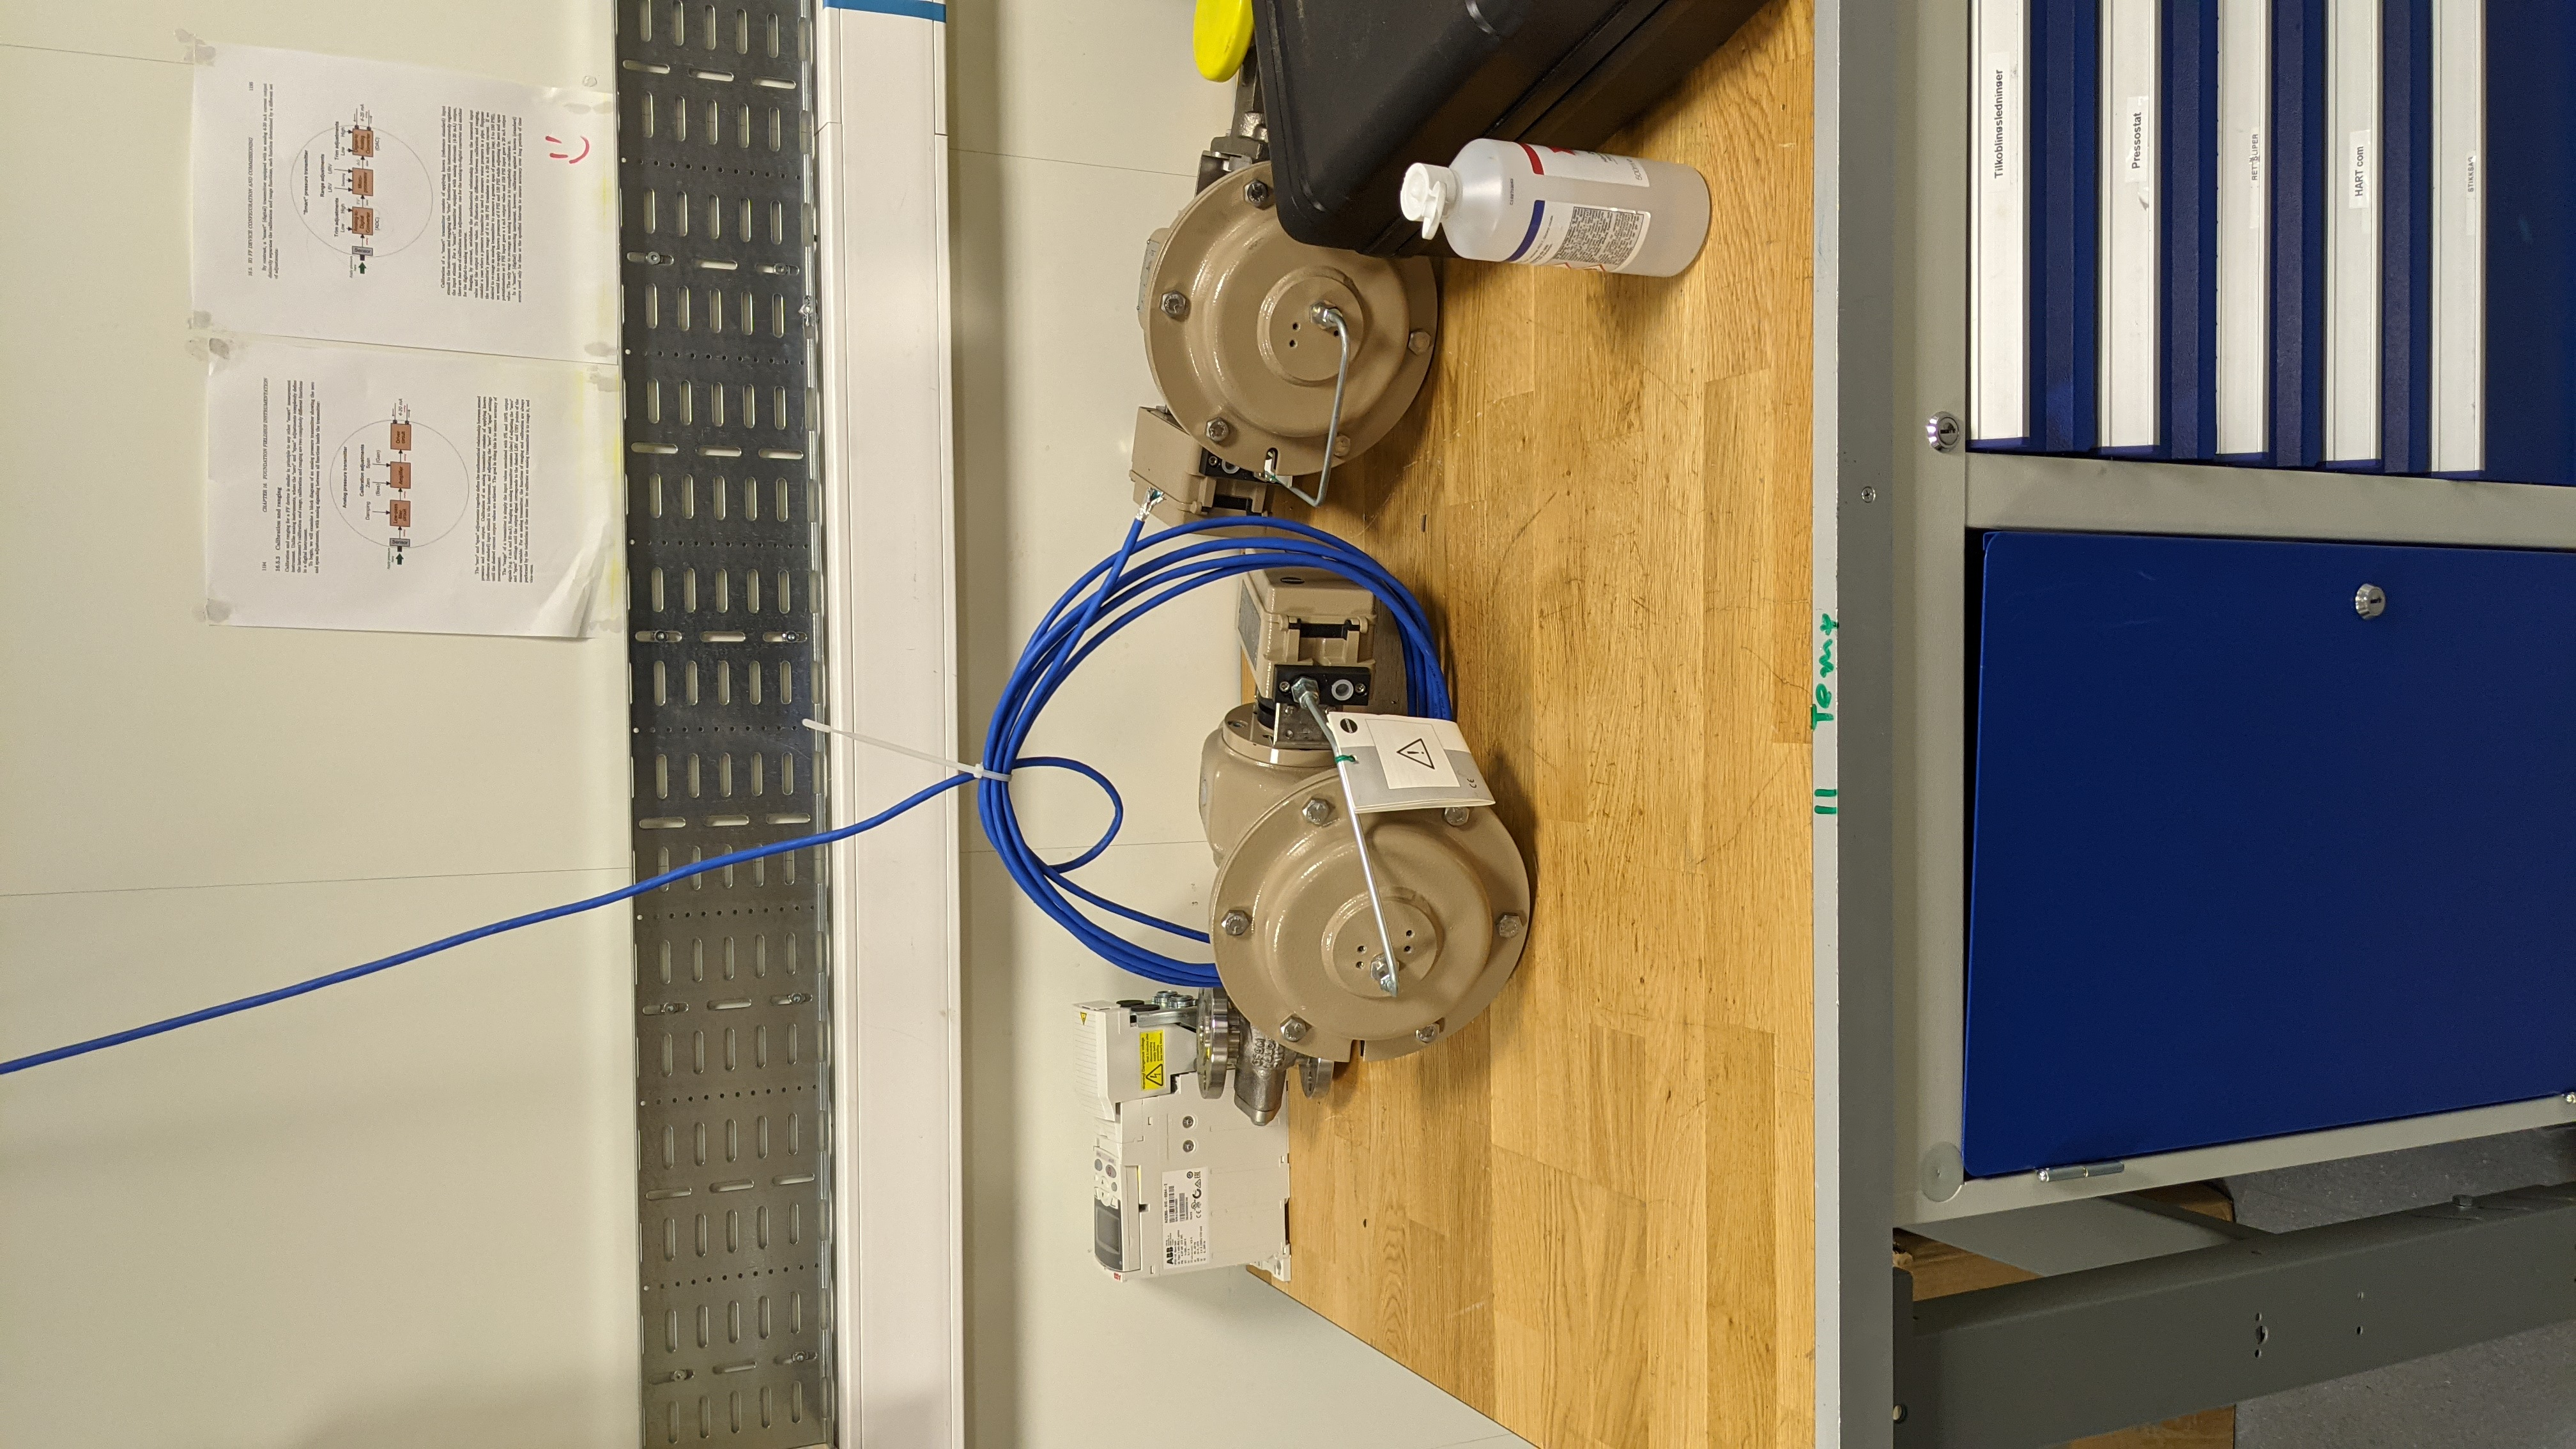
\includegraphics[width=10.5cm,angle=-90]{stasjon11x01.jpg}$$

Stasjon 11 er for benkkalibrering av temperatursensorer. 

\section{Stasjon 12}

$$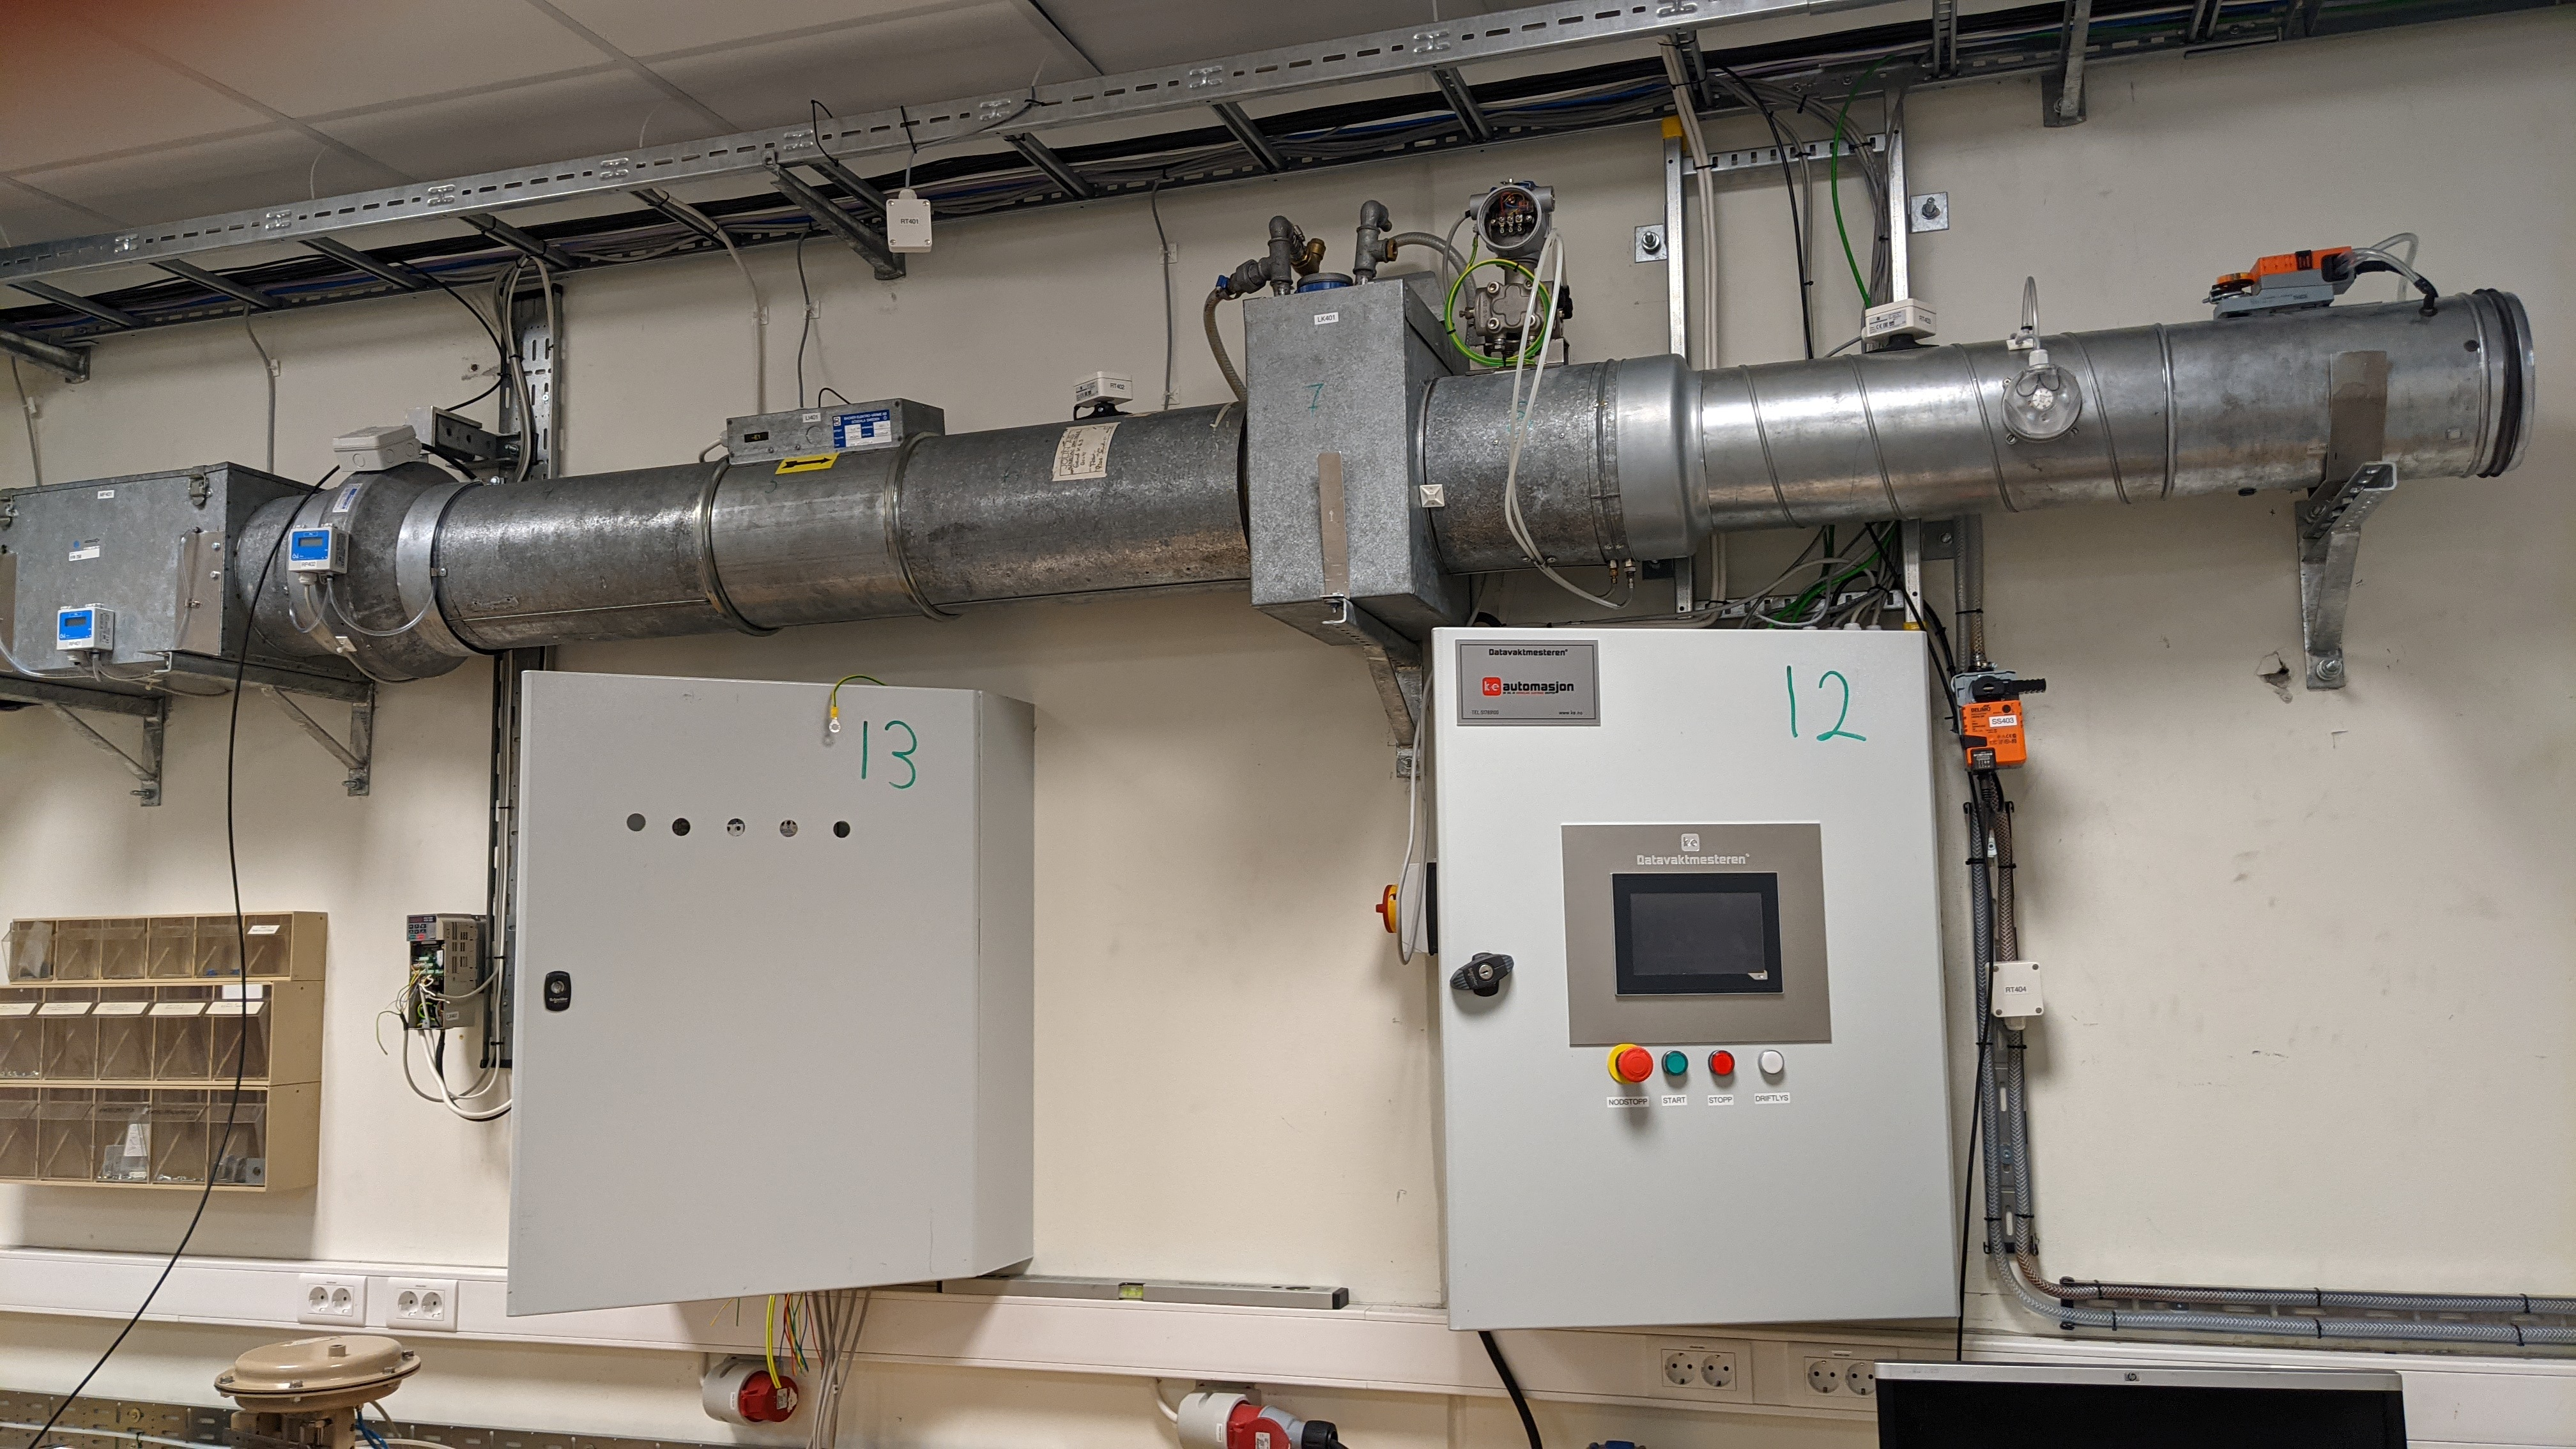
\includegraphics[width=10.5cm]{stasjon12x01.jpg}$$

Stasjon 12 er et ventilasjonsaregat der instrumenteringen er gitt til oss av KE Automasjon. Denne stasjonen brukes til øvelser på sensorer og pådragsorganer som normalt byrukes i byggautomasjon og programmeringsøvelser på ukjent PLS. På stasjonen står det en B\&R PLS, denne følger standarden EN 61131-3 for prgrammering av pls. Det vil si at den har mange likeheter med programmering i Codesys. 
\section{Stasjon 13}

$$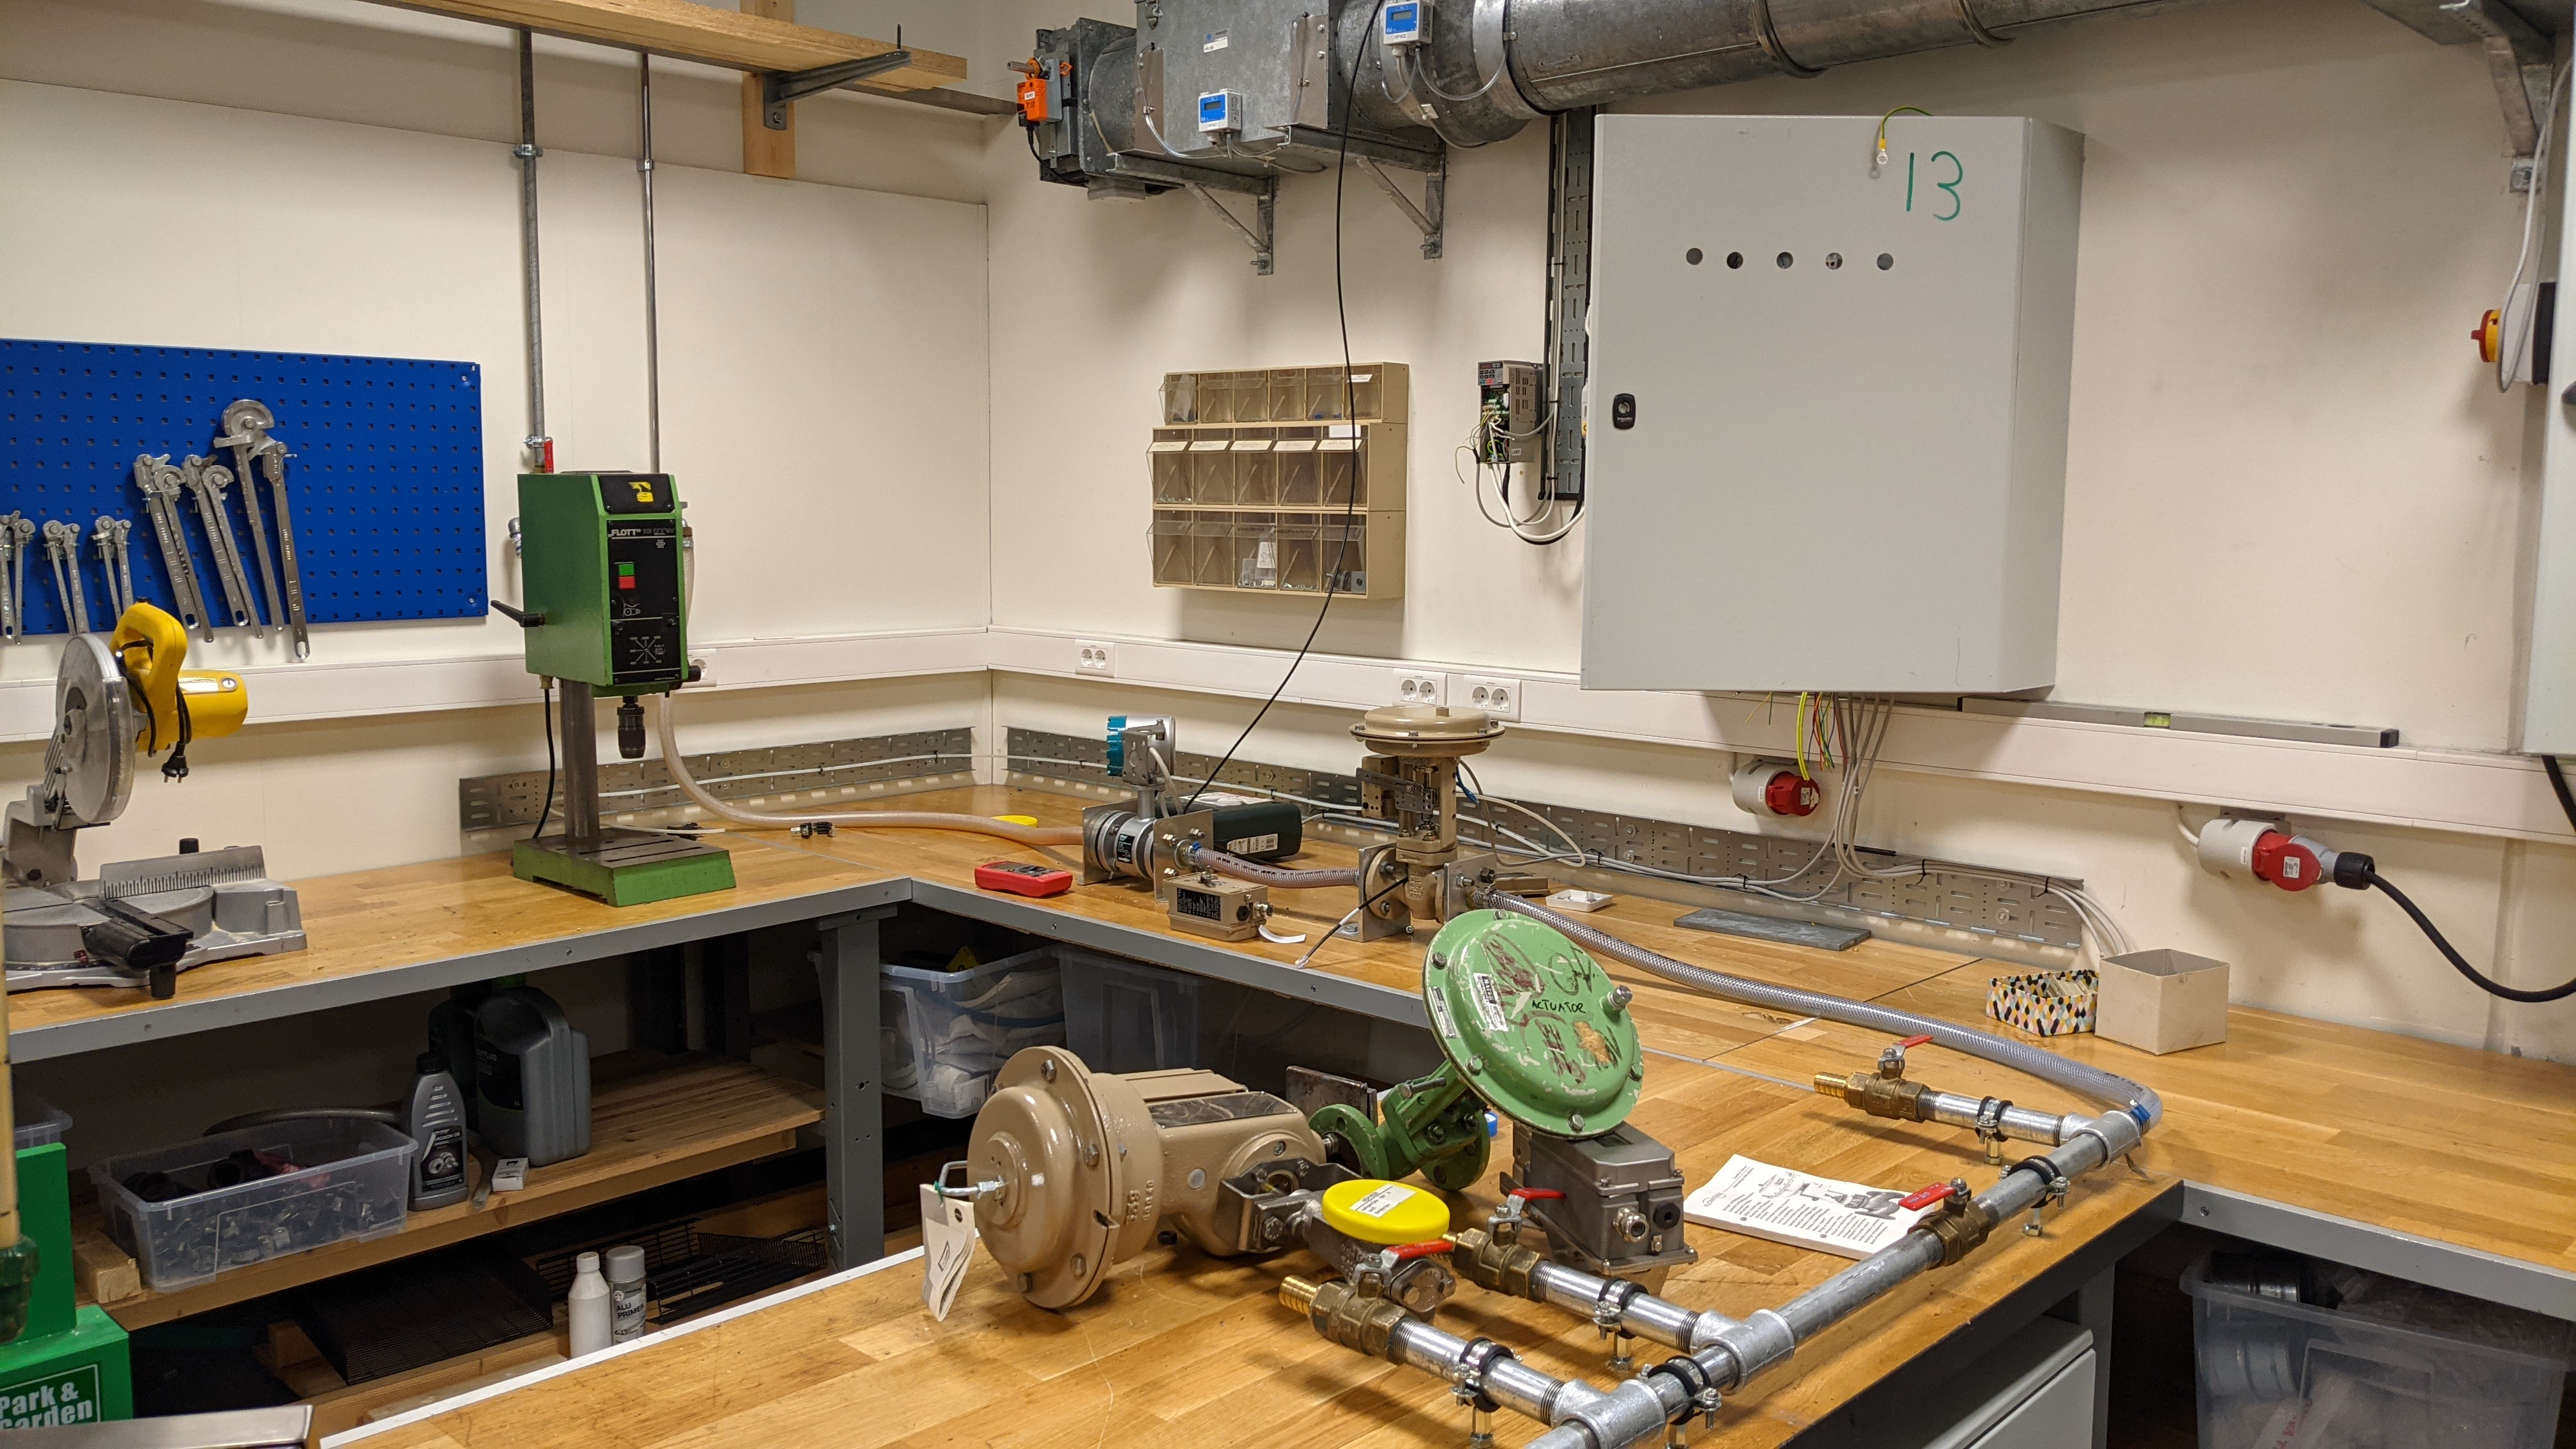
\includegraphics[width=10.5cm]{stasjon13x01.jpg}$$


\section{Stasjon 14}

$$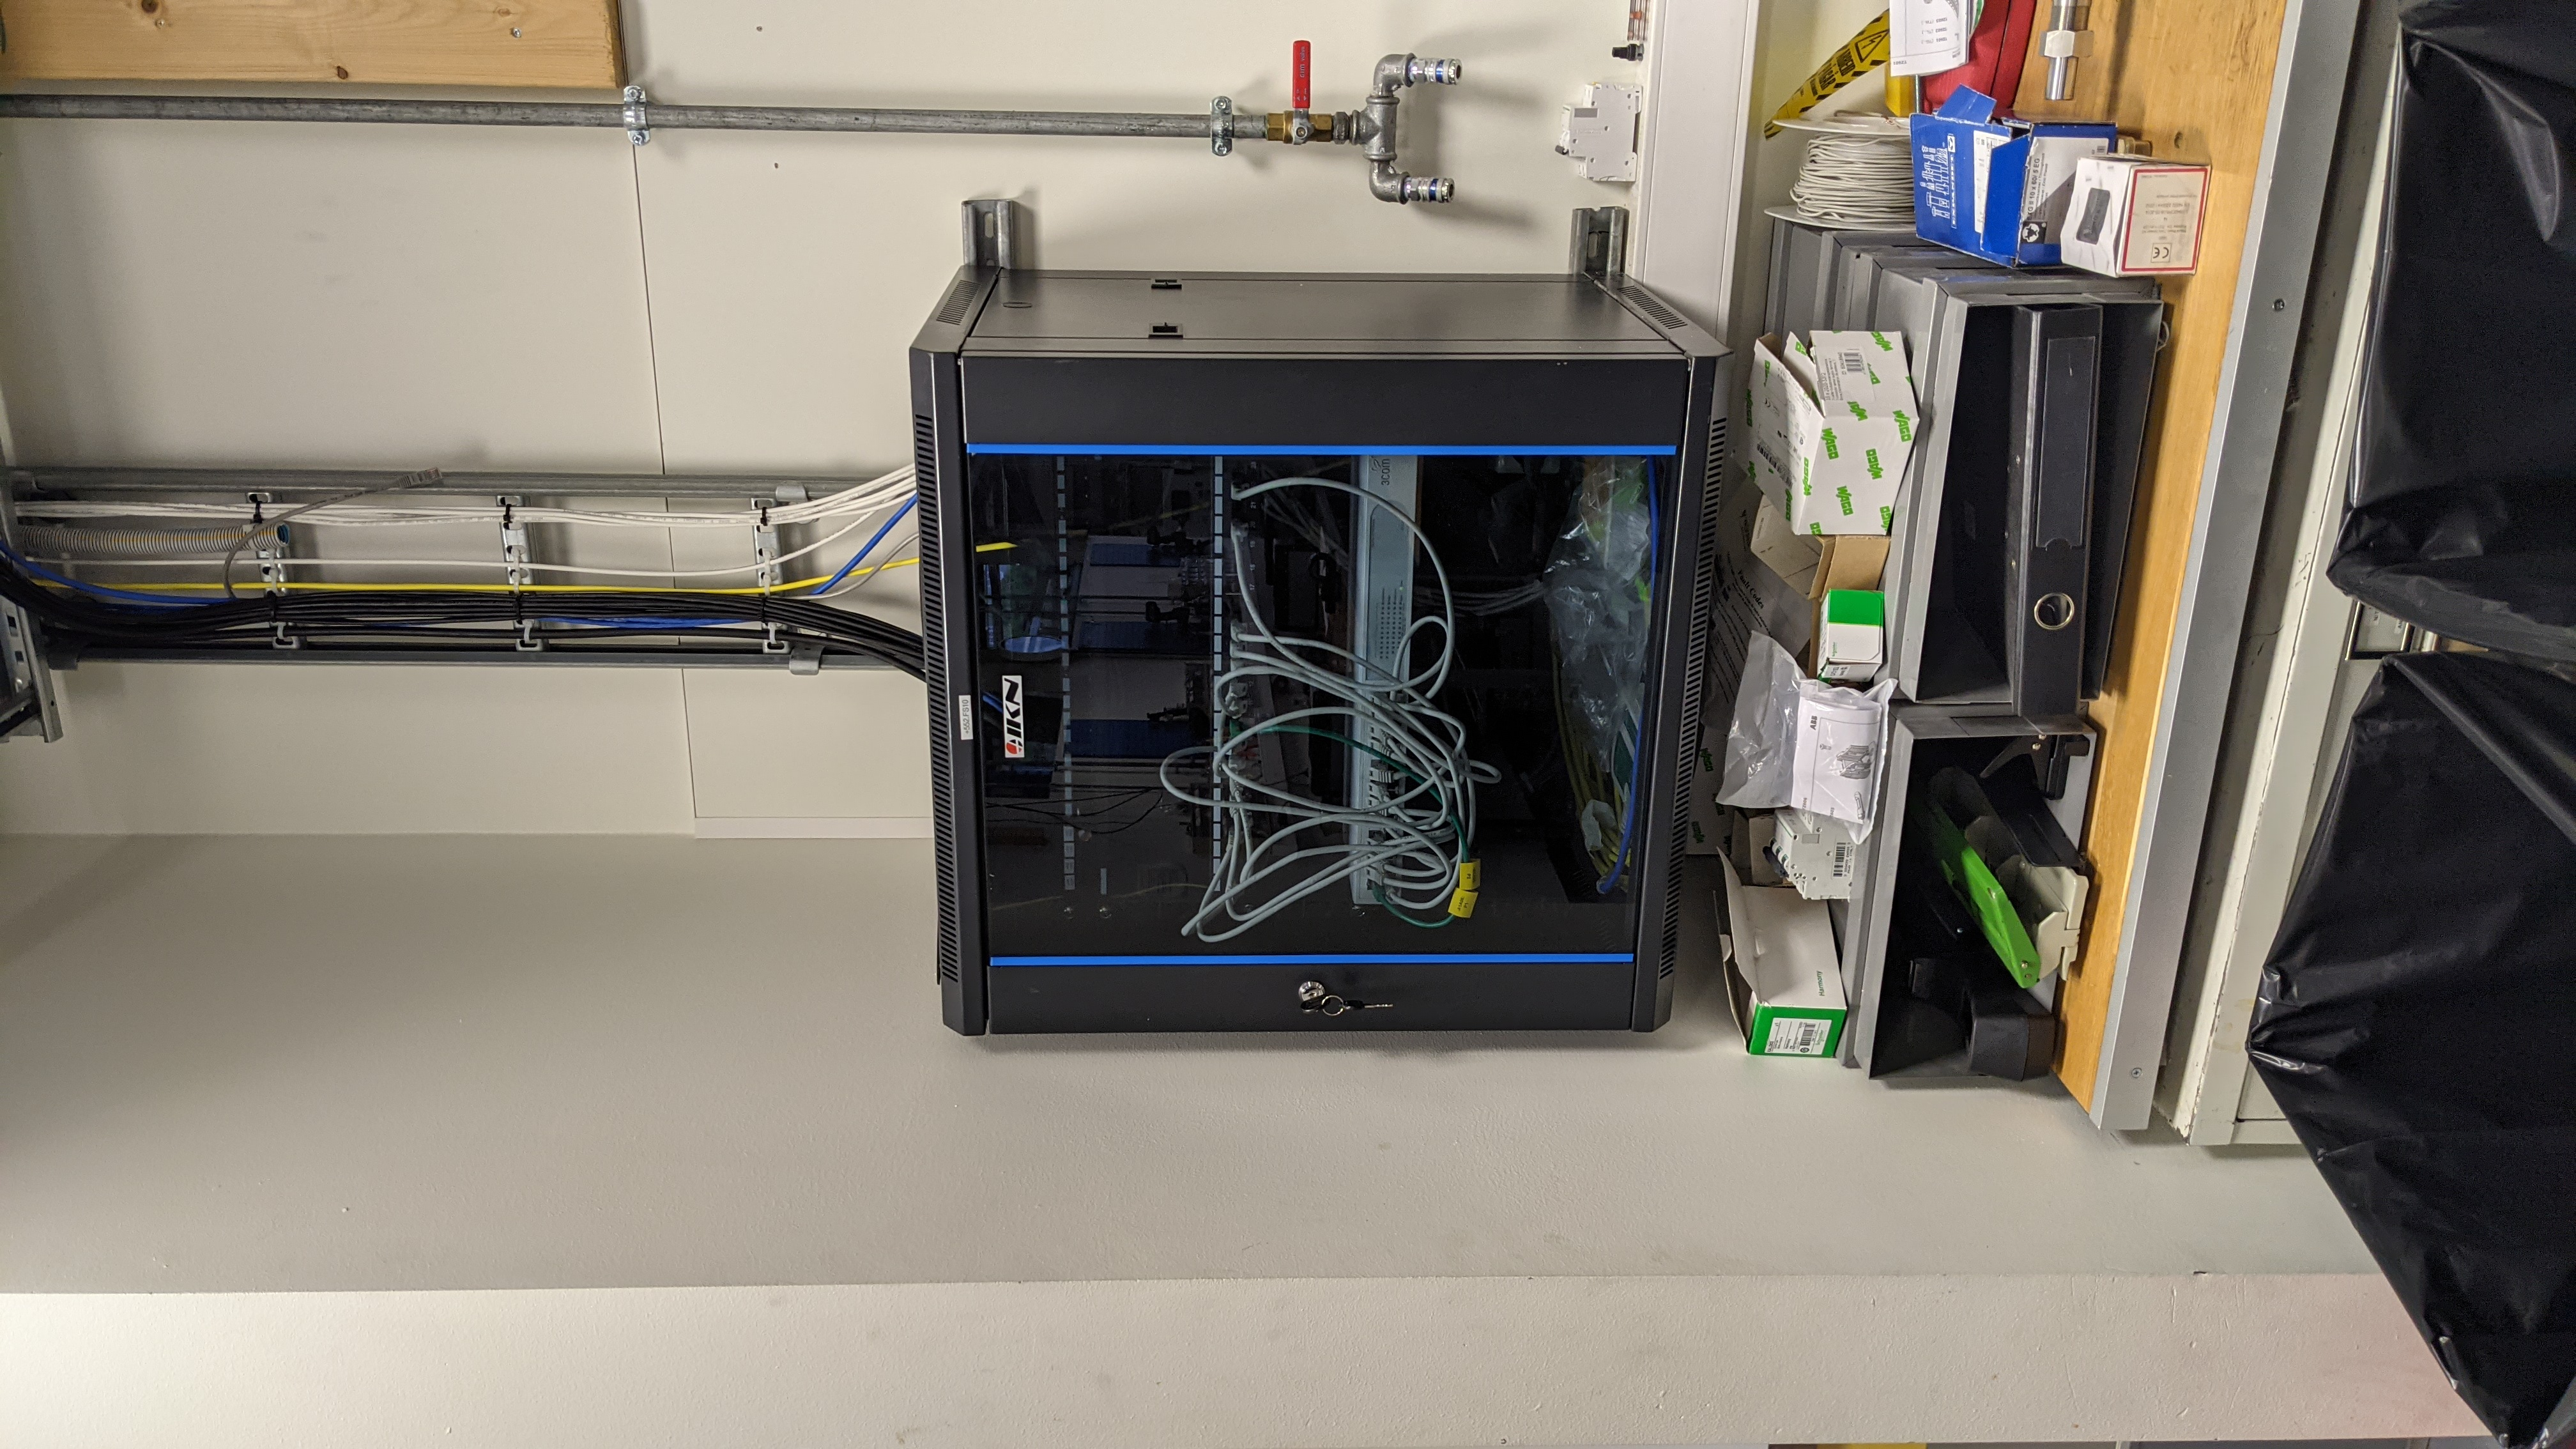
\includegraphics[width=10.5cm,angle=-90]{stasjon14x01.jpg}$$


\section{Stasjon 15}

$$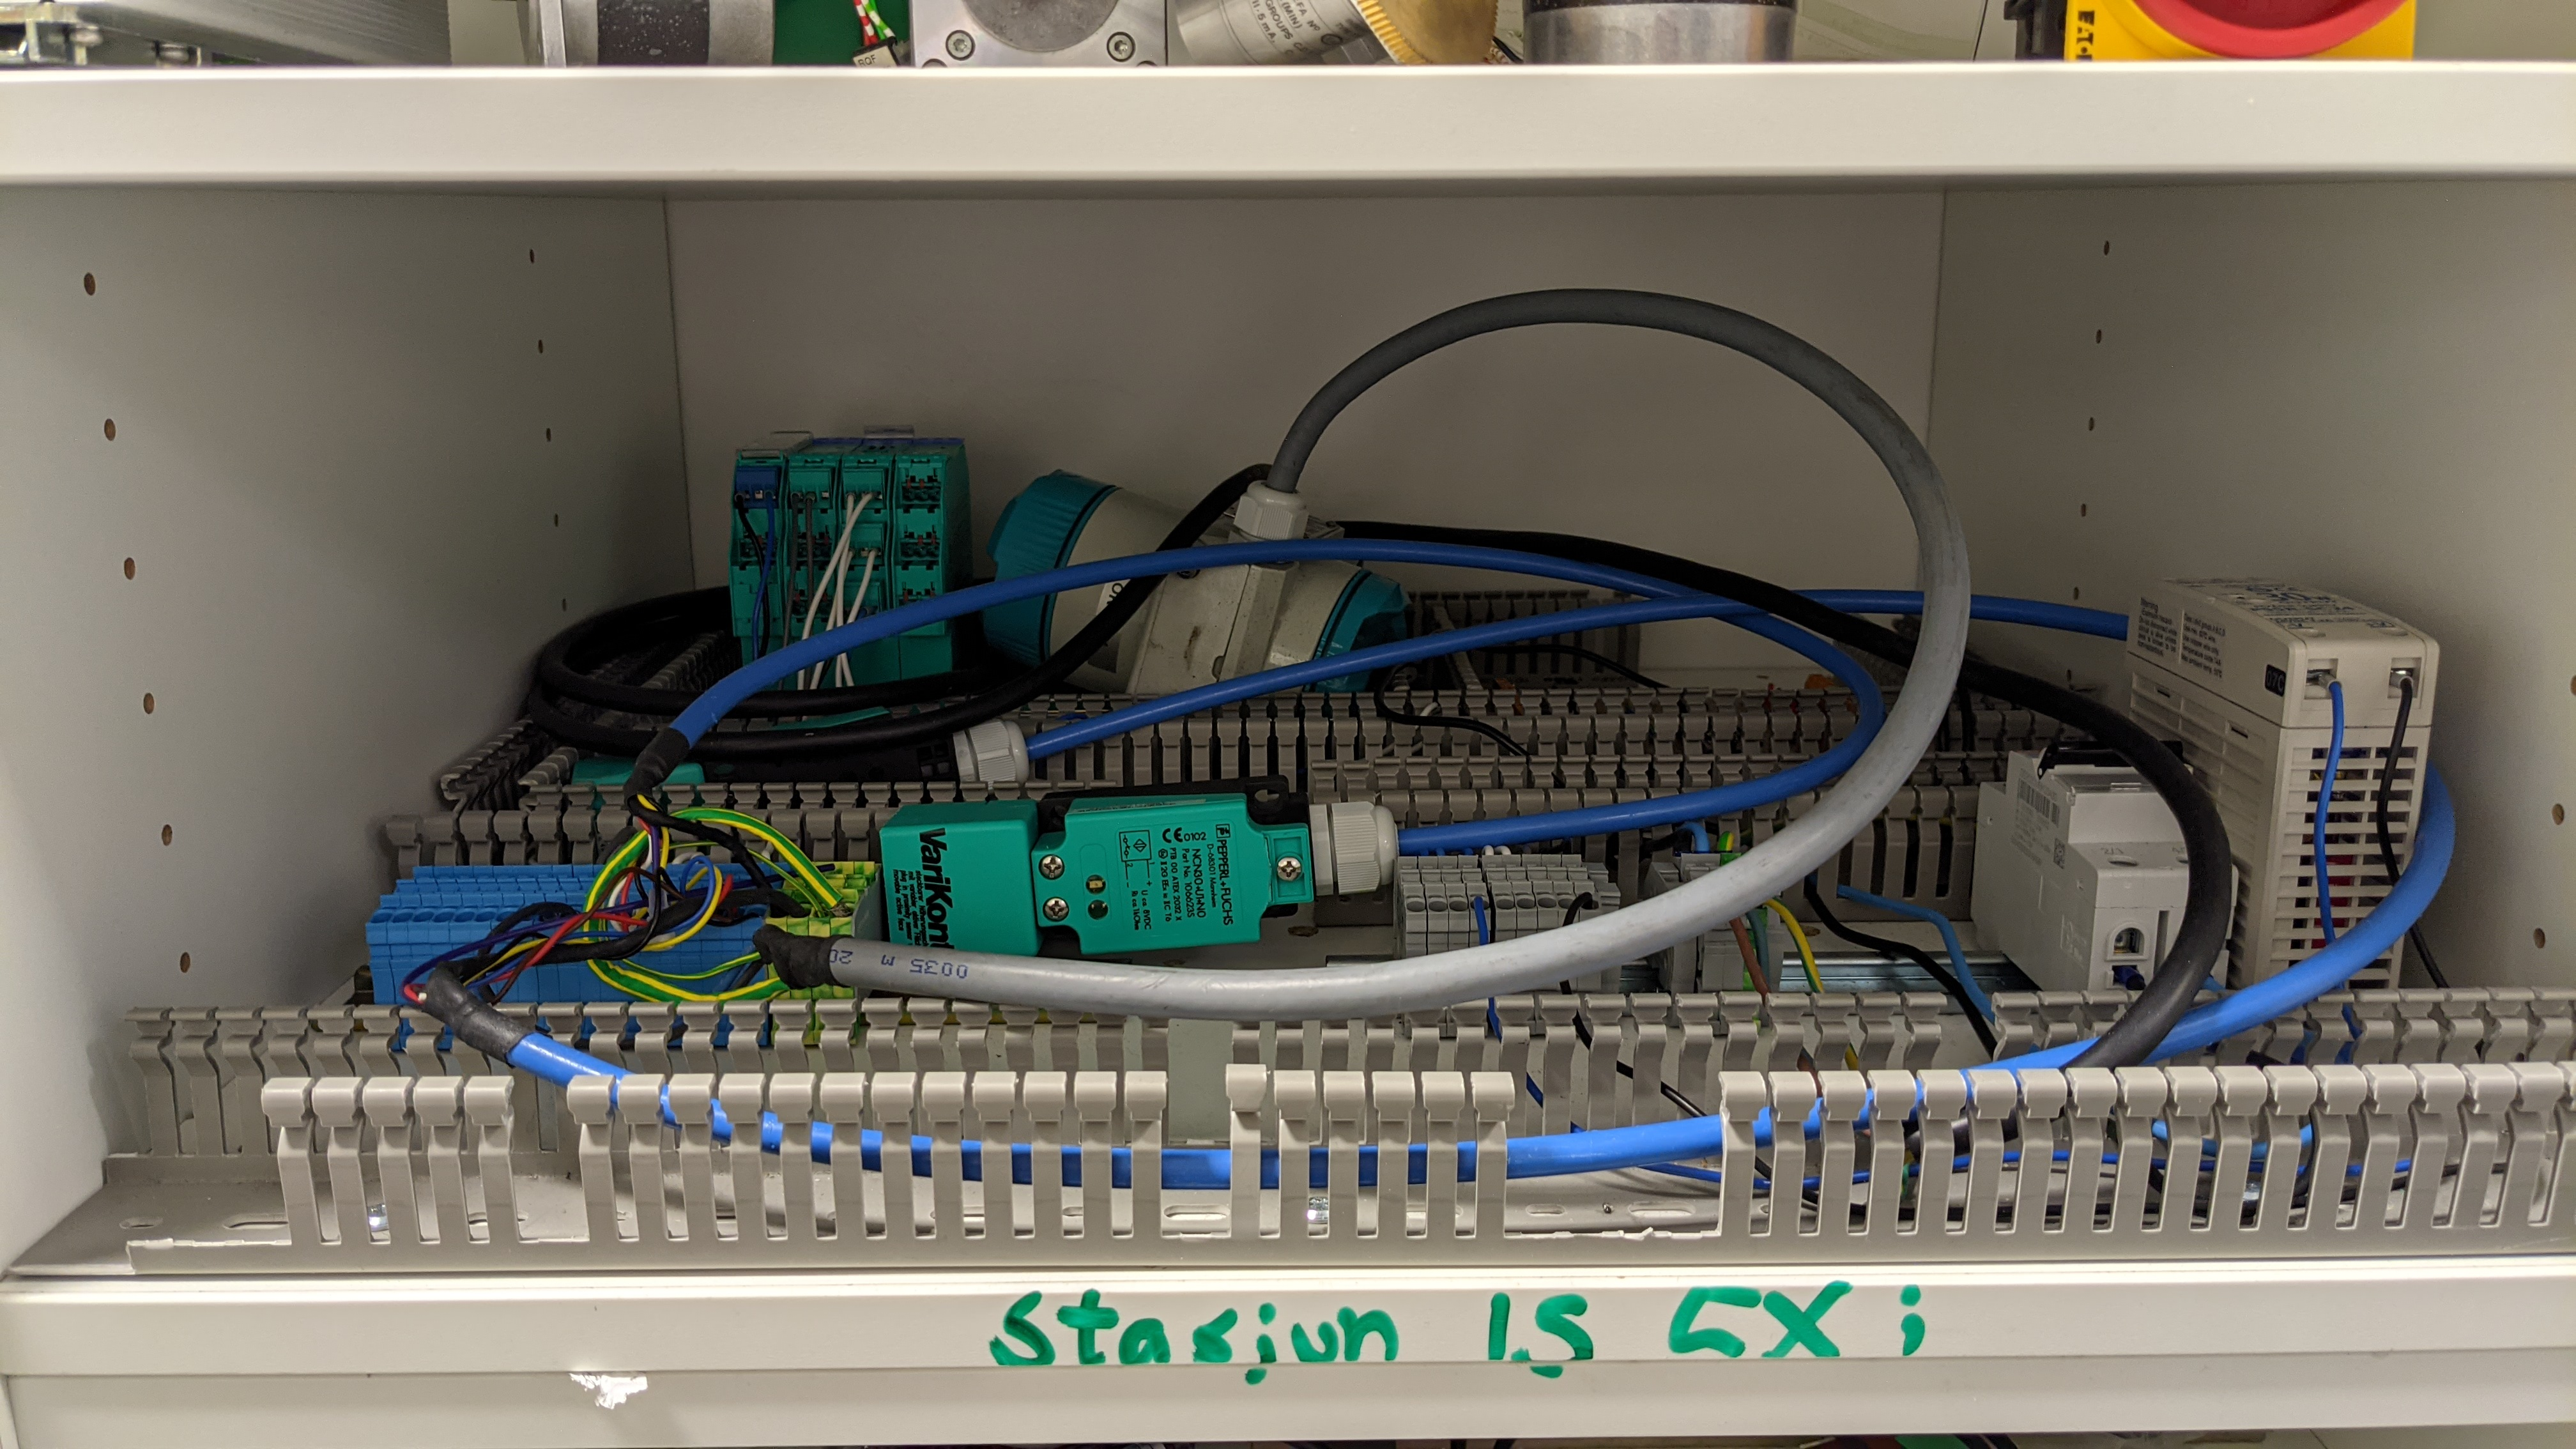
\includegraphics[width=10.5cm]{stasjon15x01.jpg}$$


\section{Stasjon 16}

$$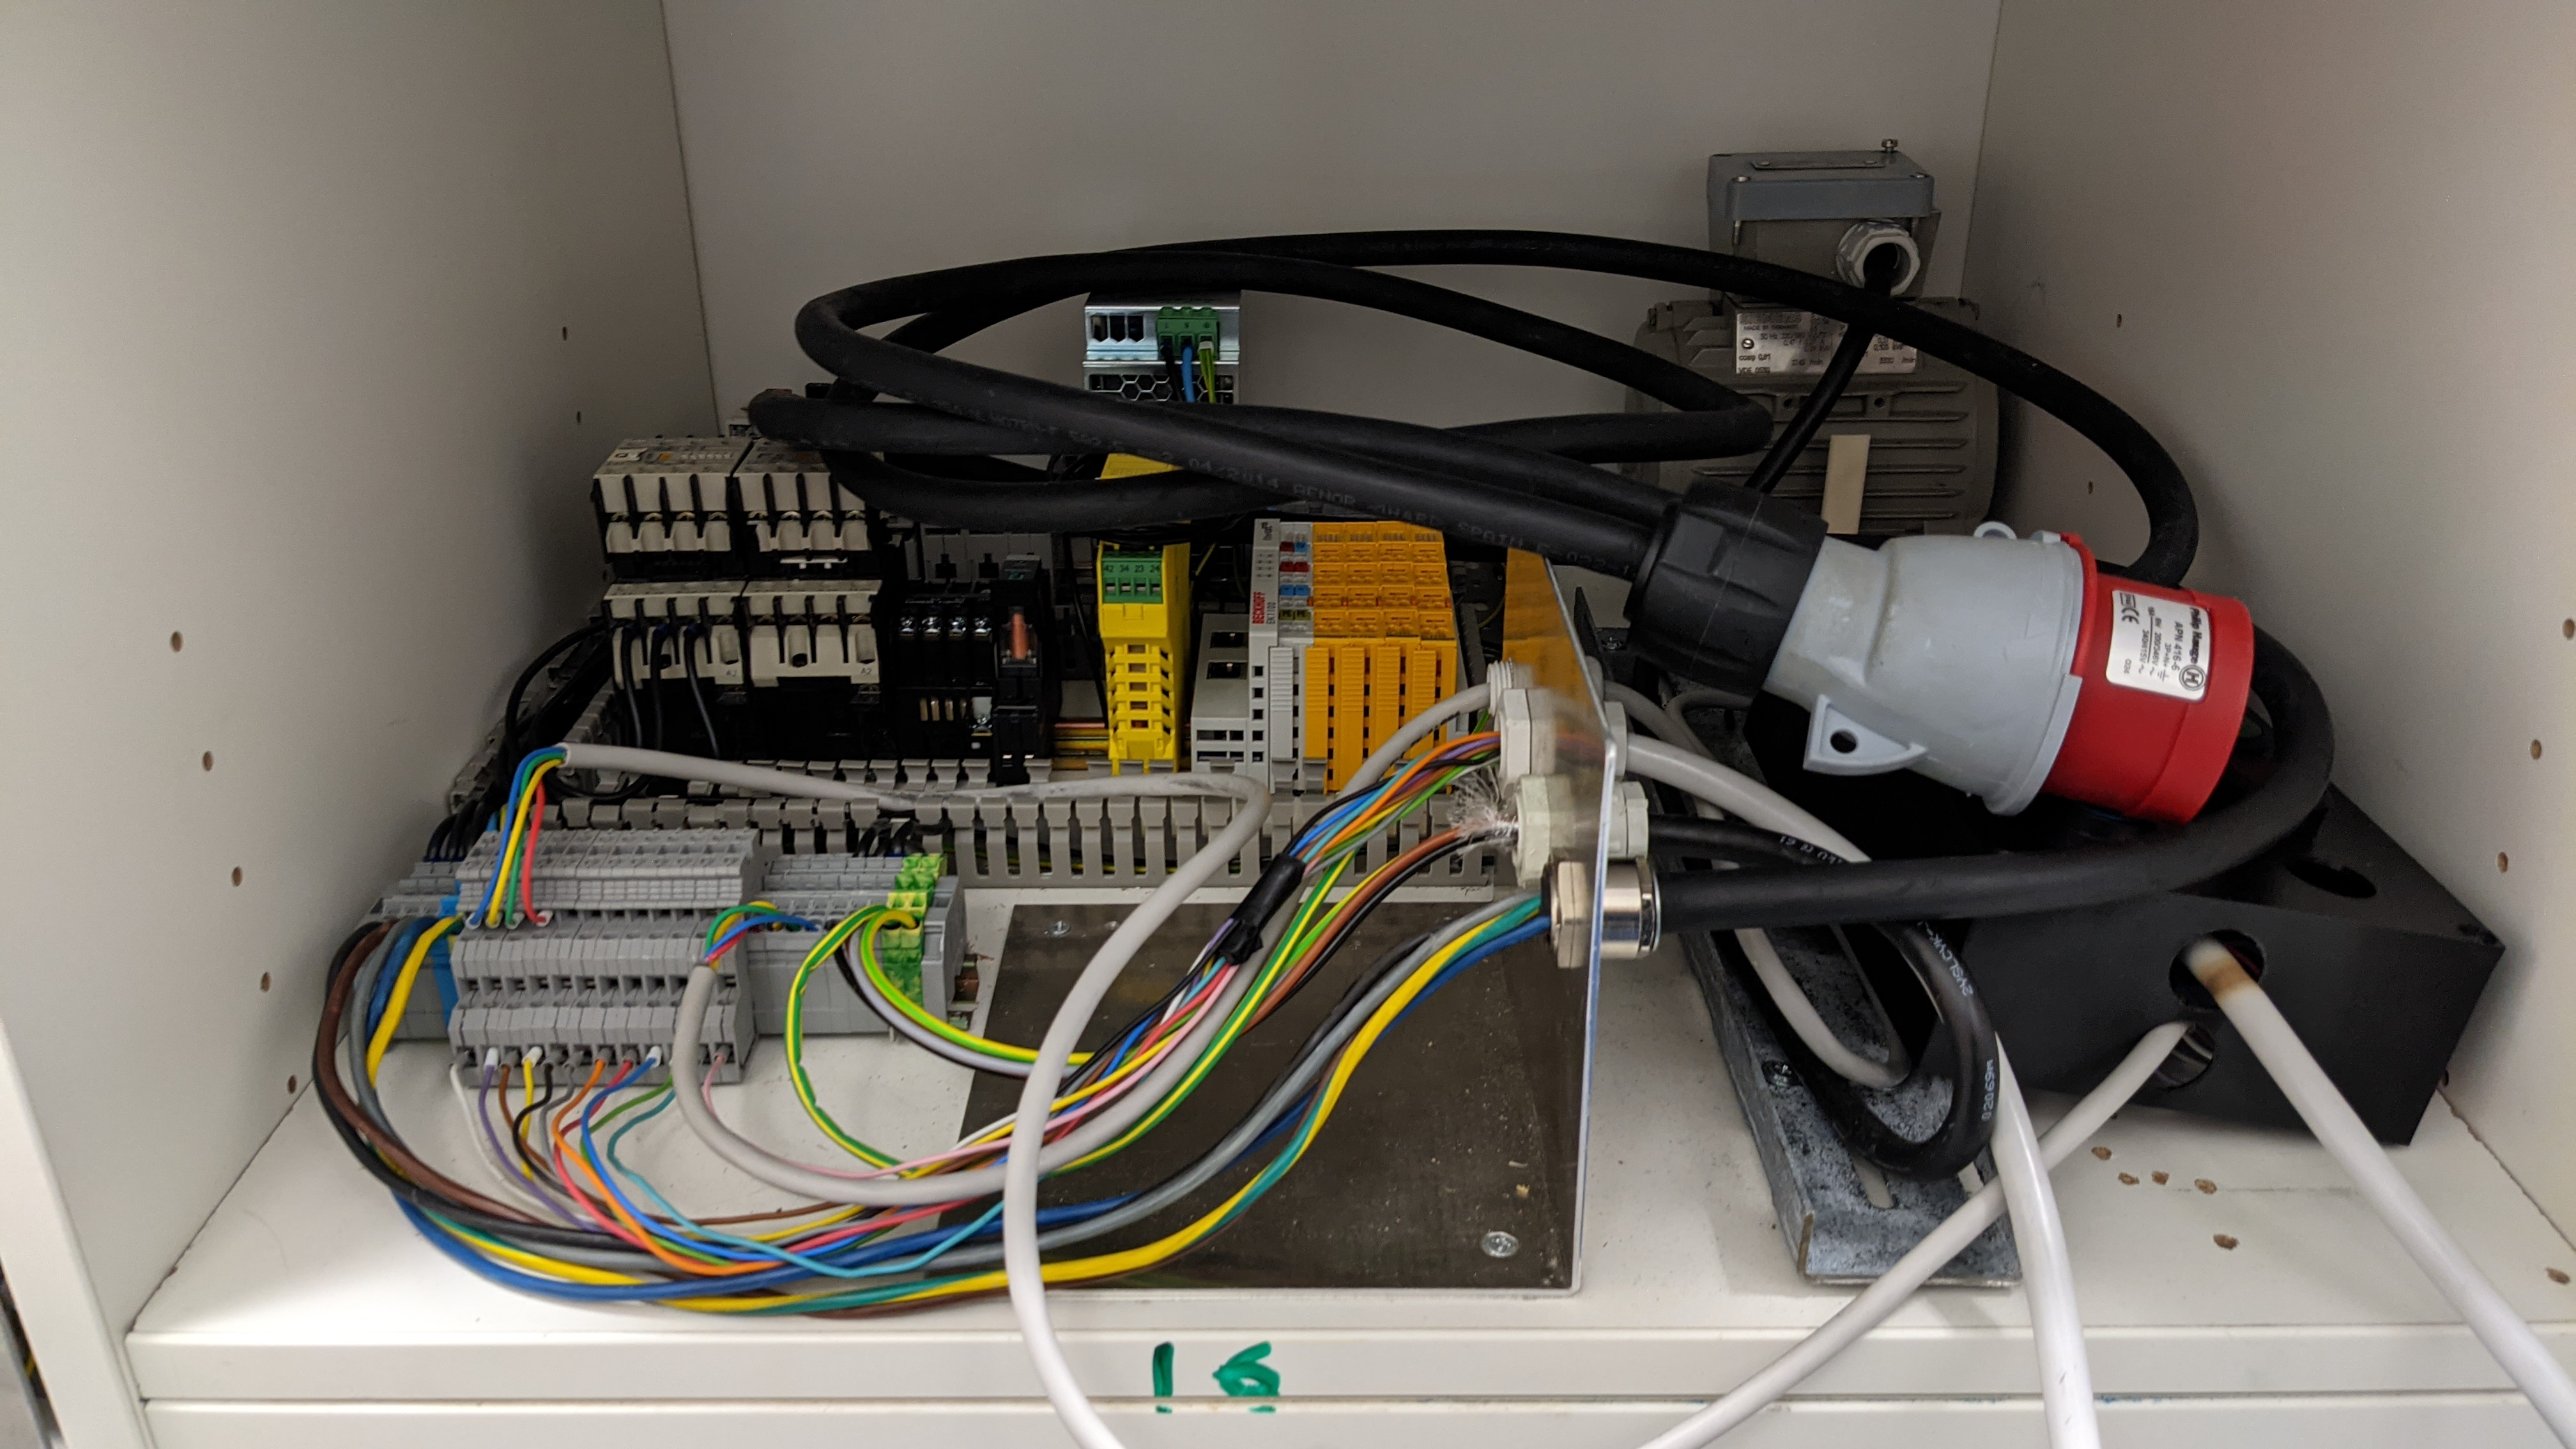
\includegraphics[width=10.5cm]{stasjon16x01.jpg}$$


\section{Stasjon 17}

$$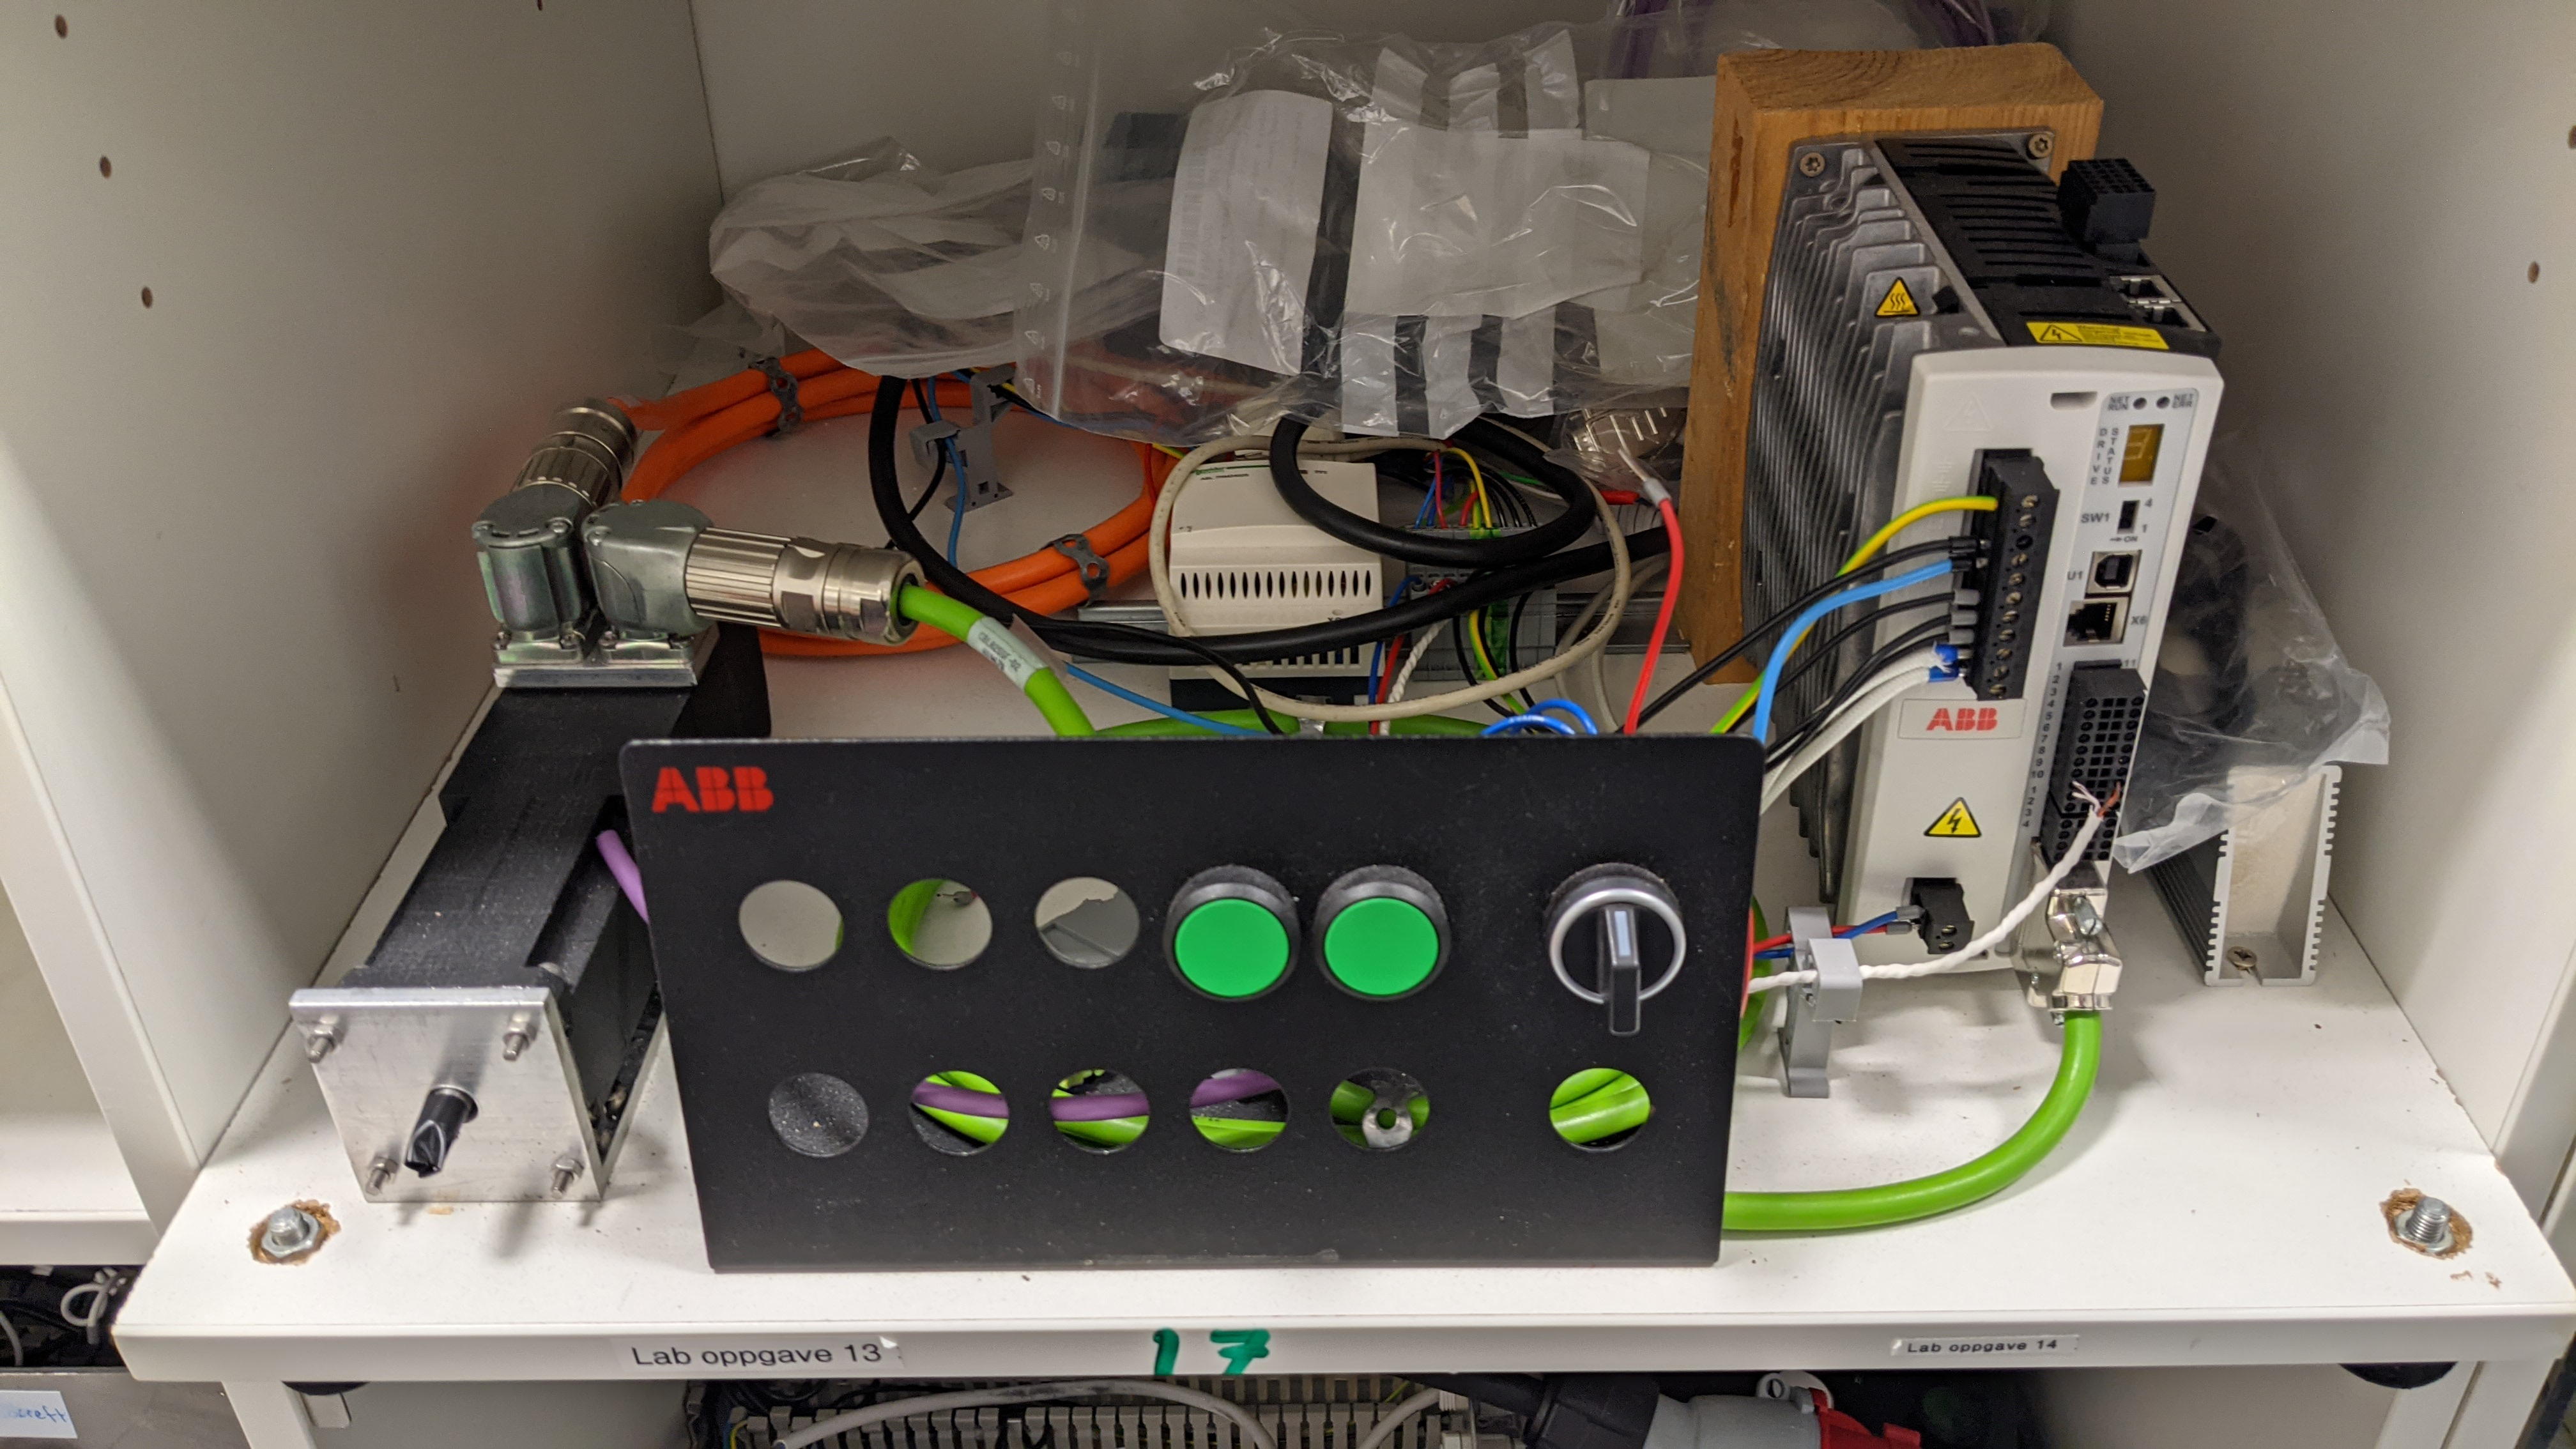
\includegraphics[width=10.5cm]{stasjon17x01.jpg}$$


\section{Stasjon 18}

$$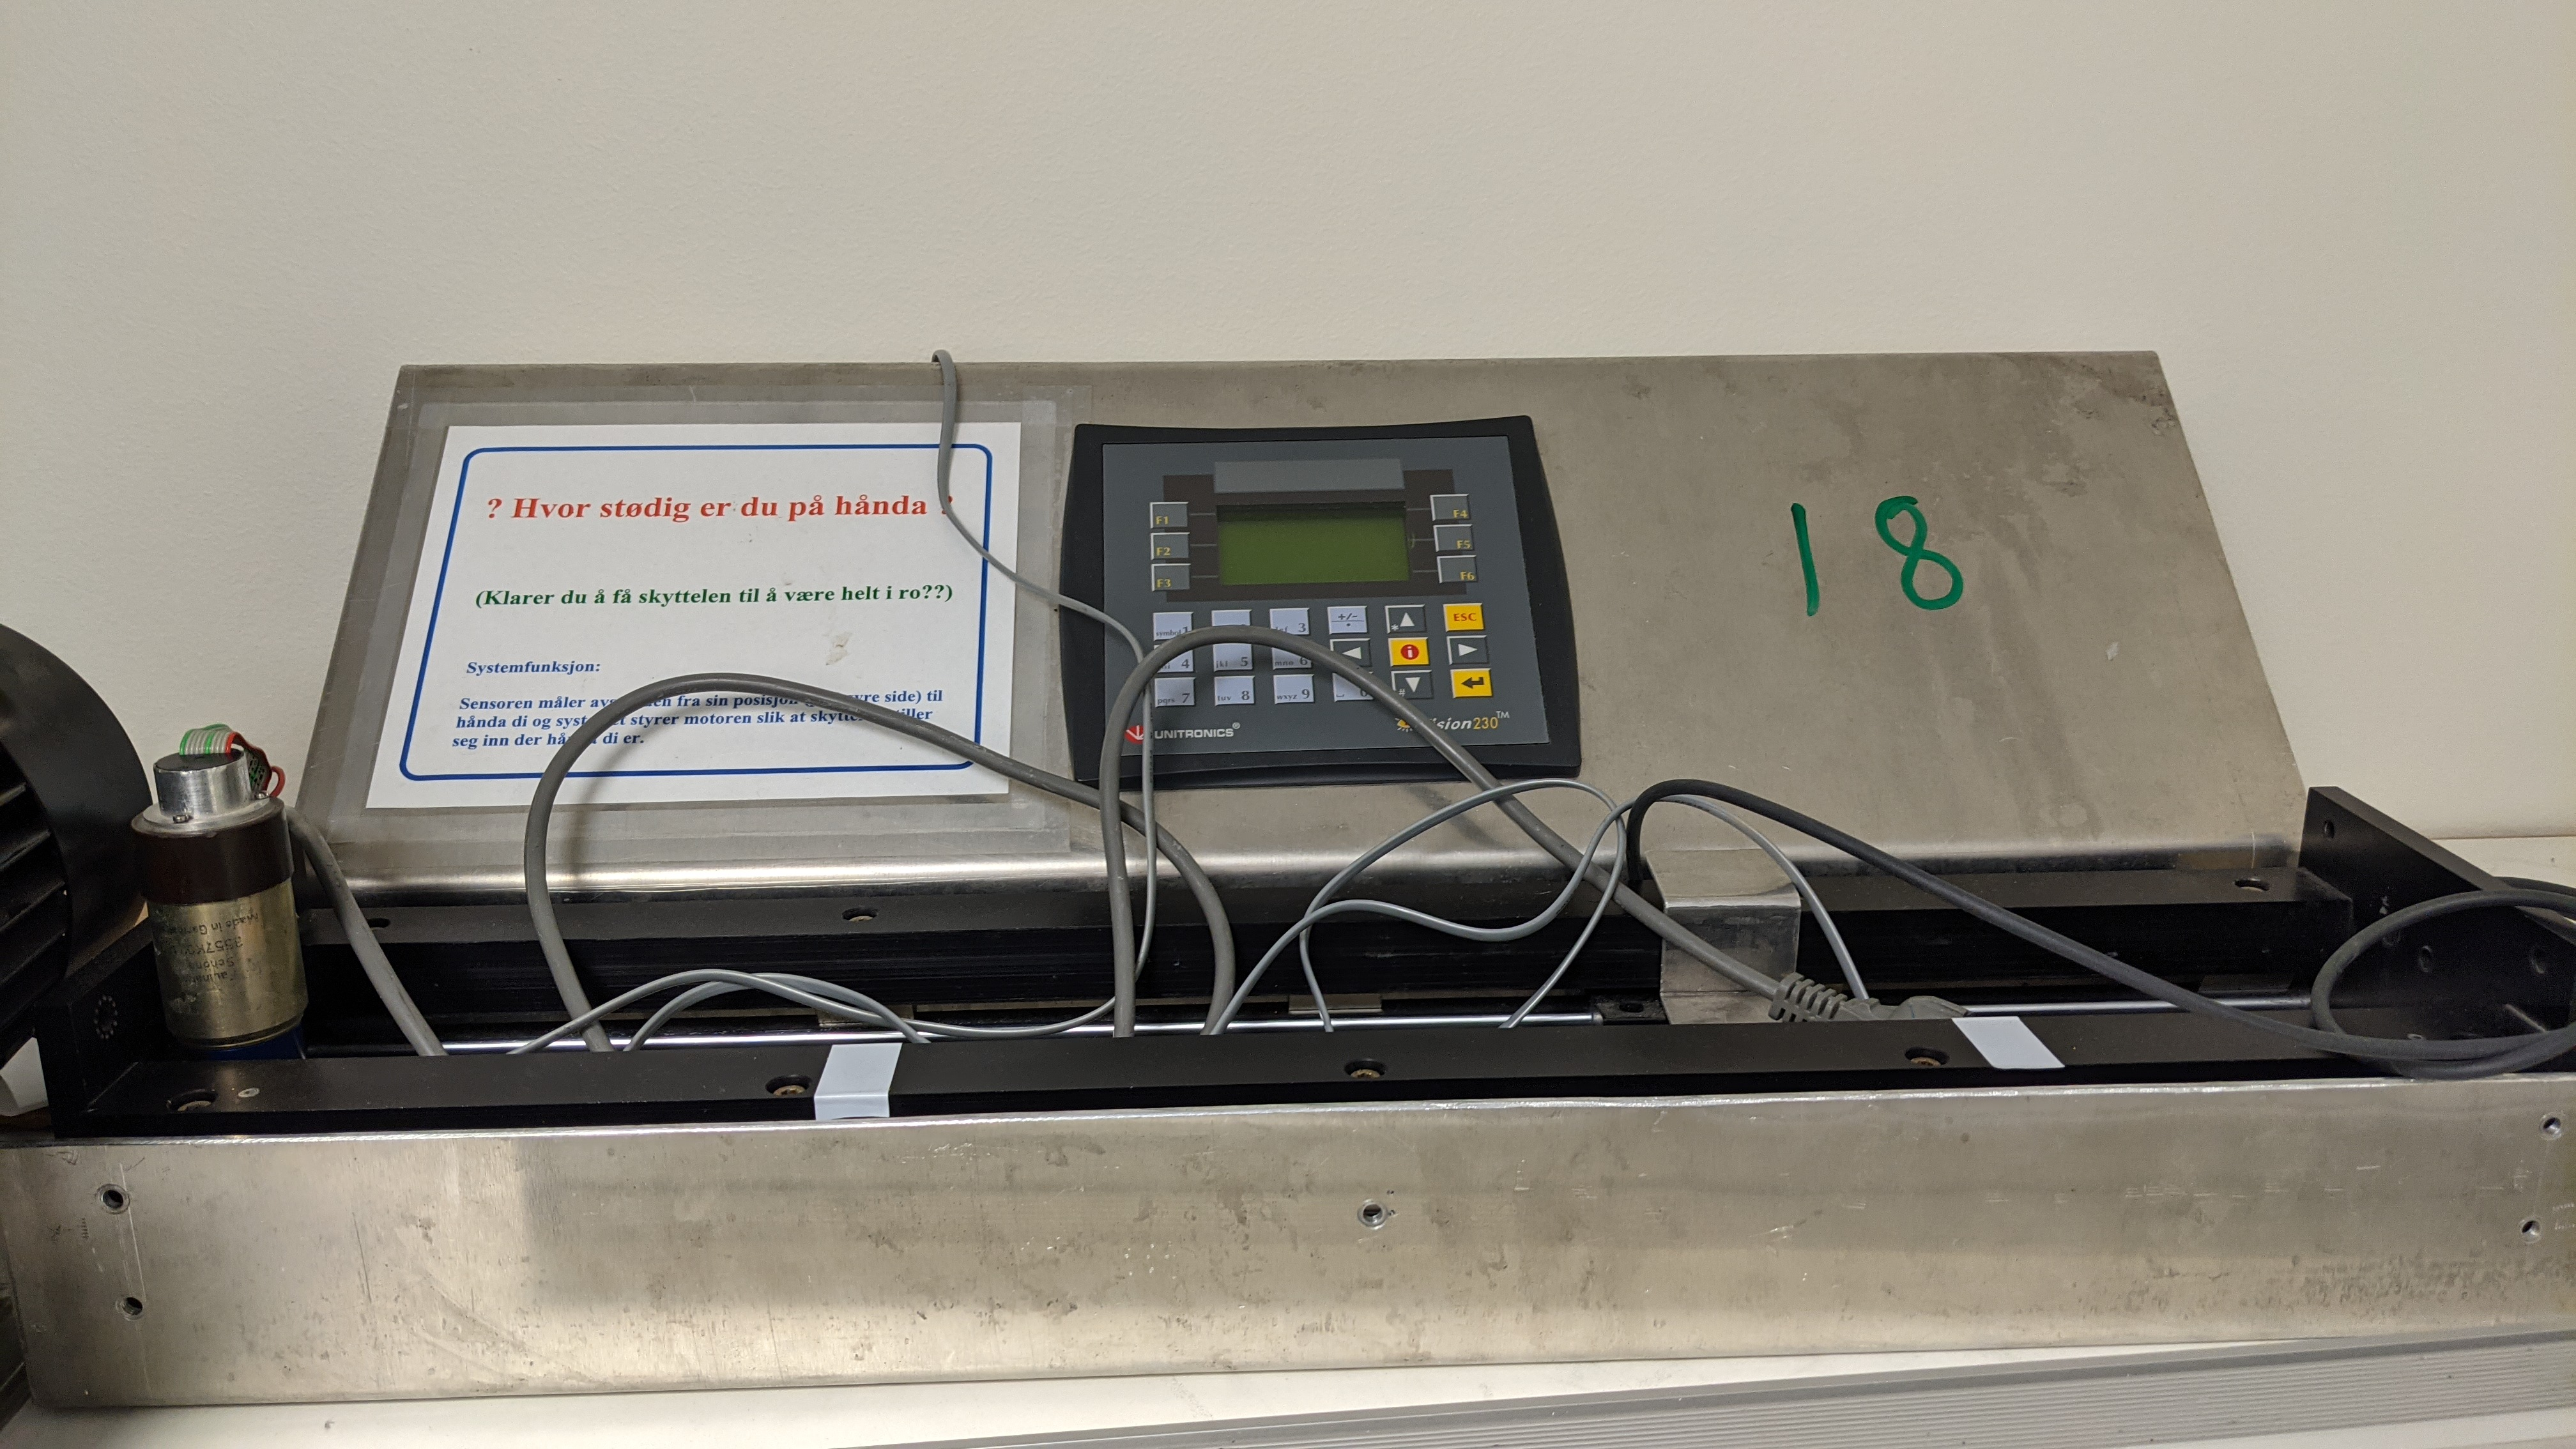
\includegraphics[width=10.5cm]{stasjon18x01.jpg}$$


\section{Stasjon 19}

$$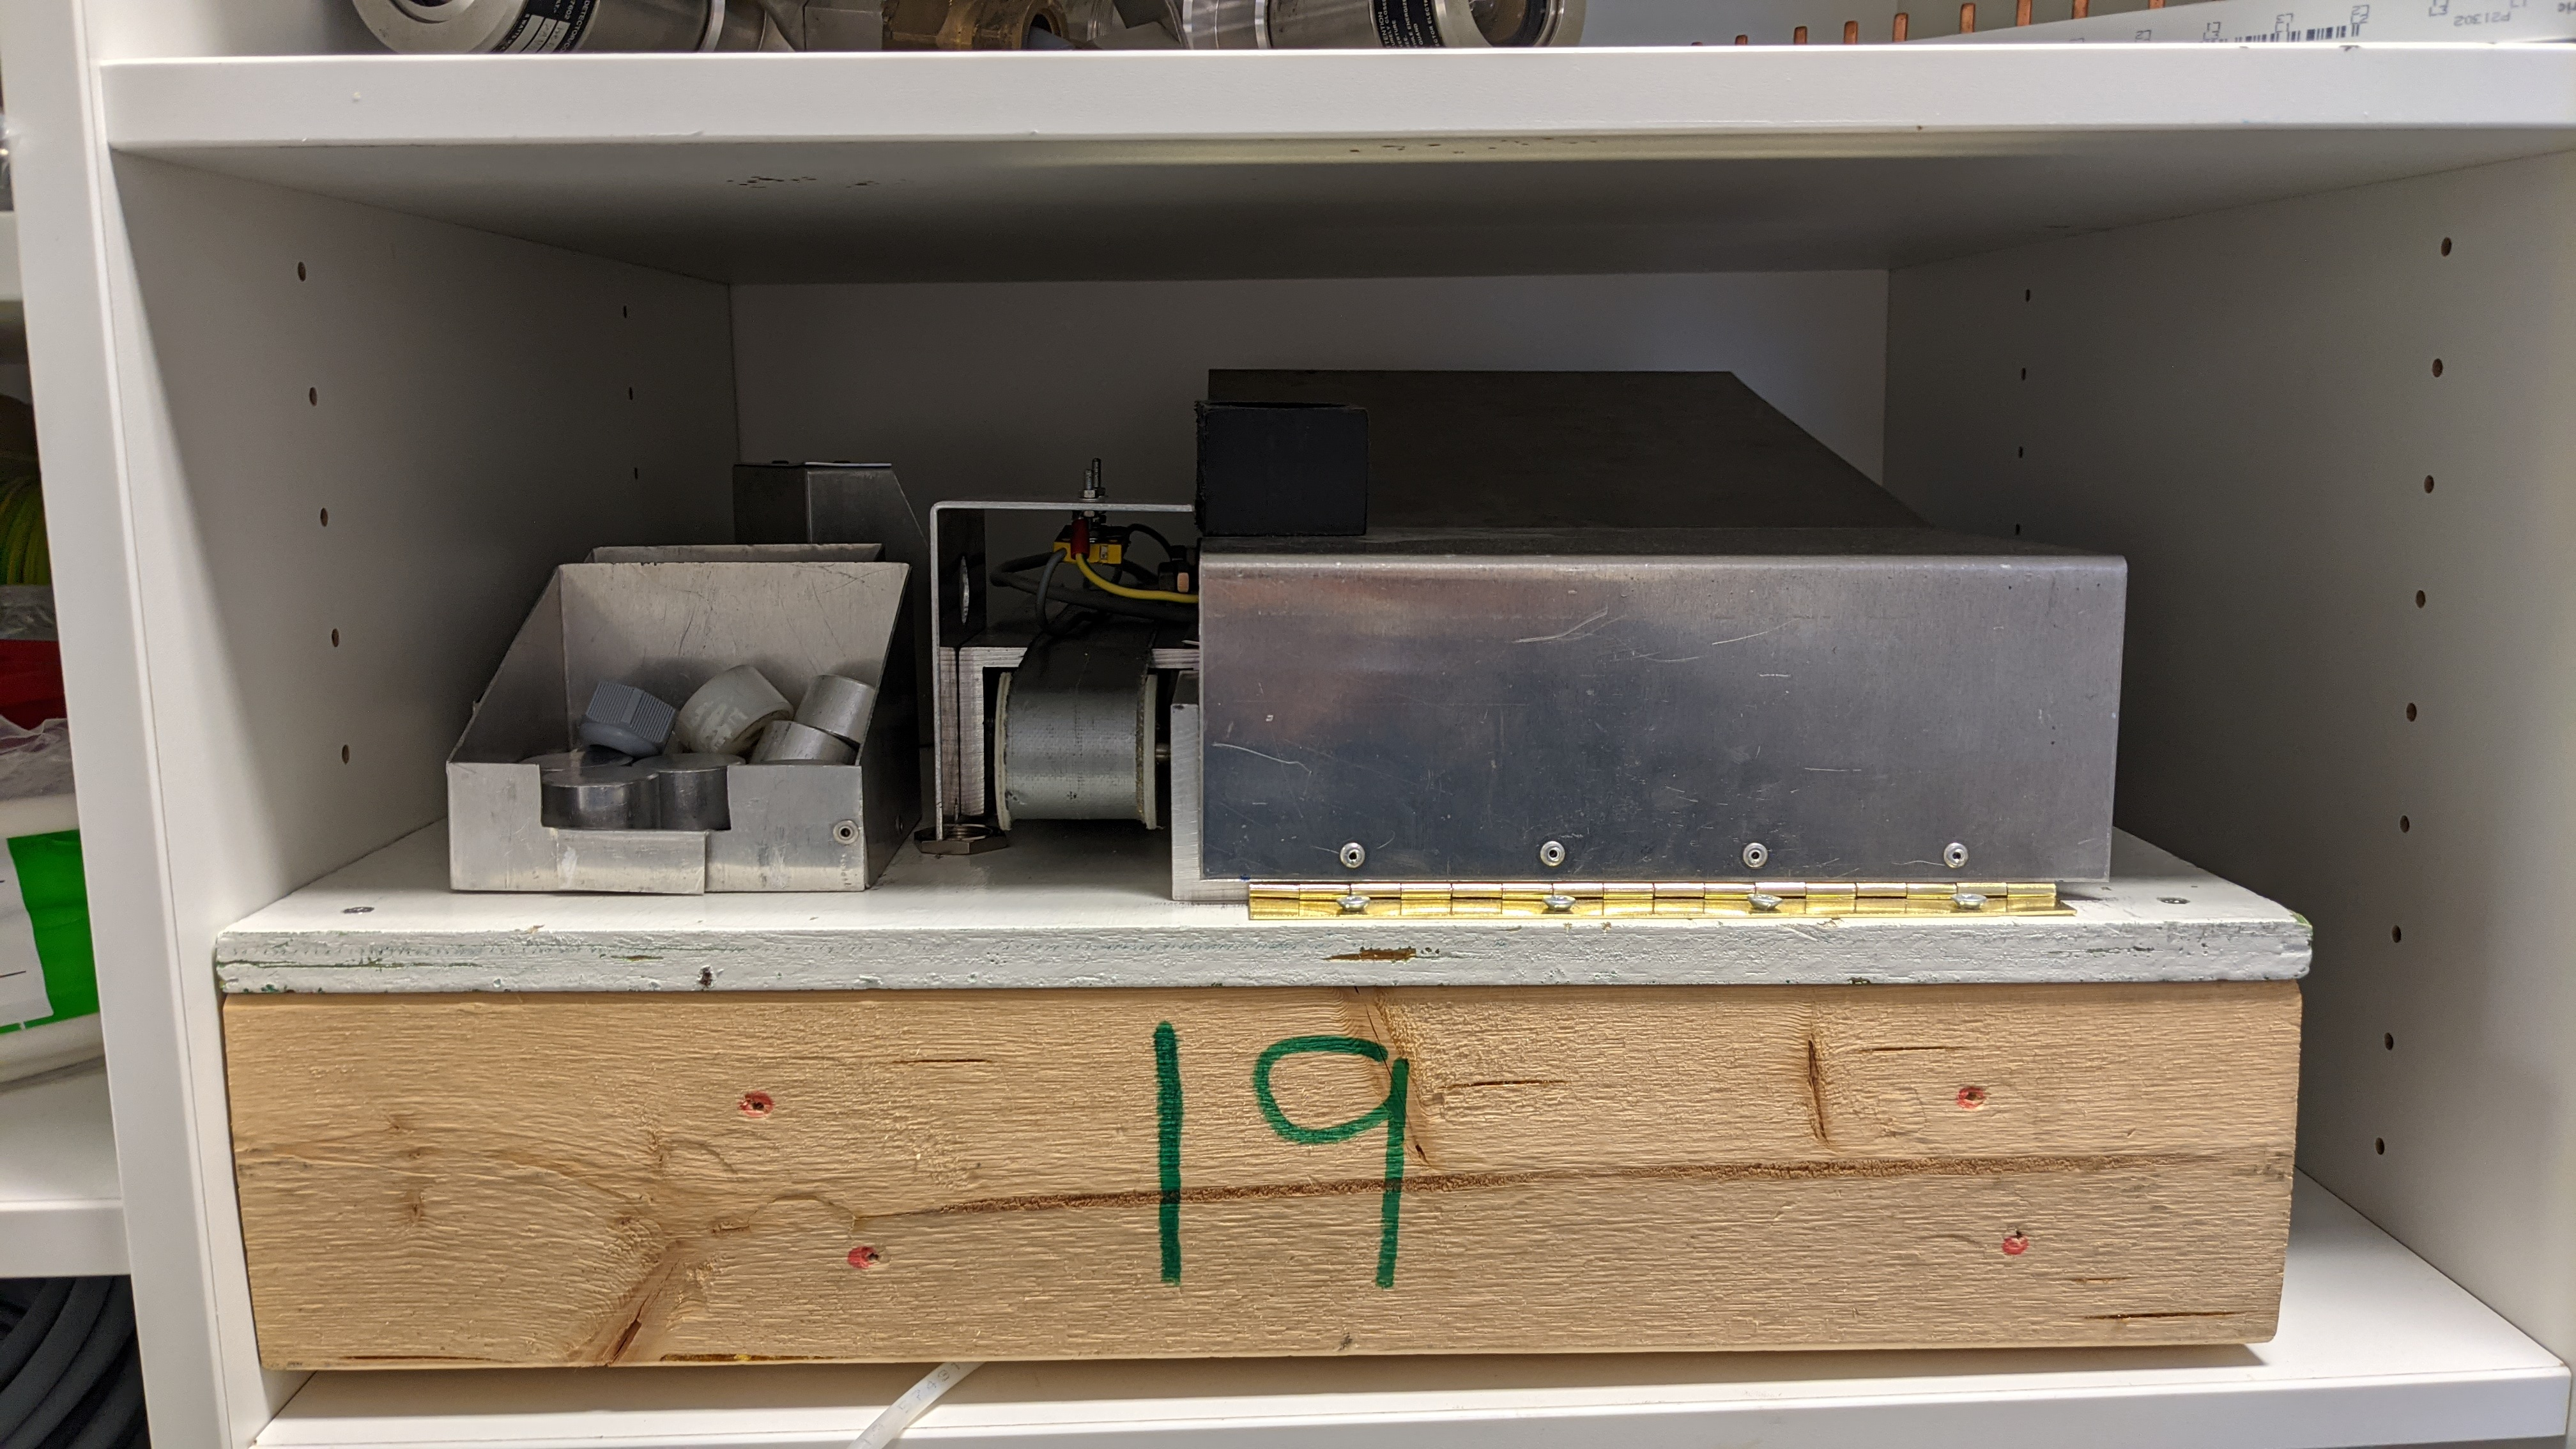
\includegraphics[width=10.5cm]{stasjon19x01.jpg}$$











































\end{document}


